% This is "sig-alternate.tex" V2.1 April 2013
% This file should be compiled with V2.5 of "sig-alternate.cls" May 2012
%
% This example file demonstrates the use of the 'sig-alternate.cls'
% V2.5 LaTeX2e document class file. It is for those submitting
% articles to ACM Conference Proceedings WHO DO NOT WISH TO
% STRICTLY ADHERE TO THE SIGS (PUBS-BOARD-ENDORSED) STYLE.
% The 'sig-alternate.cls' file will produce a similar-looking,
% albeit, 'tighter' paper resulting in, invariably, fewer pages.
%
% ----------------------------------------------------------------------------------------------------------------
% This .tex file (and associated .cls V2.5) produces:
%       1) The Permission Statement
%       2) The Conference (location) Info information
%       3) The Copyright Line with ACM data
%       4) NO page numbers
%
% as against the acm_proc_article-sp.cls file which
% DOES NOT produce 1) thru' 3) above.
%
% Using 'sig-alternate.cls' you have control, however, from within
% the source .tex file, over both the CopyrightYear
% (defaulted to 200X) and the ACM Copyright Data
% (defaulted to X-XXXXX-XX-X/XX/XX).
% e.g.
% \CopyrightYear{2007} will cause 2007 to appear in the copyright line.
% \crdata{0-12345-67-8/90/12} will cause 0-12345-67-8/90/12 to appear in the copyright line.
%
% ---------------------------------------------------------------------------------------------------------------
% This .tex source is an example which *does* use
% the .bib file (from which the .bbl file % is produced).
% REMEMBER HOWEVER: After having produced the .bbl file,
% and prior to final submission, you *NEED* to 'insert'
% your .bbl file into your source .tex file so as to provide
% ONE 'self-contained' source file.
%
% ================= IF YOU HAVE QUESTIONS =======================
% Questions regarding the SIGS styles, SIGS policies and
% procedures, Conferences etc. should be sent to
% Adrienne Griscti (griscti@acm.org)
%
% Technical questions _only_ to
% Gerald Murray (murray@hq.acm.org)
% ===============================================================
%
% For tracking purposes - this is V2.0 - May 2012

\documentclass{sig-alternate-05-2015}


\begin{document}

% Copyright
\setcopyright{acmcopyright}
%\setcopyright{acmlicensed}
%\setcopyright{rightsretained}
%\setcopyright{usgov}
%\setcopyright{usgovmixed}
%\setcopyright{cagov}
%\setcopyright{cagovmixed}


% DOI
\doi{10.475/123_4}

% ISBN
\isbn{123-4567-24-567/08/06}

%Conference
\conferenceinfo{EASE '17}{June 15--16, 2017, BTH - Karlskrona, Sweden}

\acmPrice{\$15.00}

%
% --- Author Metadata here ---
\conferenceinfo{EASE}{'17 BTH - Karlskrona, Sweden}
%\CopyrightYear{2007} % Allows default copyright year (20XX) to be over-ridden - IF NEED BE.
%\crdata{0-12345-67-8/90/01}  % Allows default copyright data (0-89791-88-6/97/05) to be over-ridden - IF NEED BE.
% --- End of Author Metadata ---

\title{Seeking for the formalization of Experimentation in Software Engineering: An Empirical Study\titlenote{}}
%\subtitle{[Extended Abstract]
%\titlenote{A full version of this paper is available as
%\textit{Author's Guide to Preparing ACM SIG Proceedings Using
%\LaTeX$2_\epsilon$\ and BibTeX} at
%\texttt{www.acm.org/eaddress.htm}}}
%
% You need the command \numberofauthors to handle the 'placement
% and alignment' of the authors beneath the title.
%
% For aesthetic reasons, we recommend 'three authors at a time'
% i.e. three 'name/affiliation blocks' be placed beneath the title.
%
% NOTE: You are NOT restricted in how many 'rows' of
% "name/affiliations" may appear. We just ask that you restrict
% the number of 'columns' to three.
%
% Because of the available 'opening page real-estate'
% we ask you to refrain from putting more than six authors
% (two rows with three columns) beneath the article title.
% More than six makes the first-page appear very cluttered indeed.
%
% Use the \alignauthor commands to handle the names
% and affiliations for an 'aesthetic maximum' of six authors.
% Add names, affiliations, addresses for
% the seventh etc. author(s) as the argument for the
% \additionalauthors command.
% These 'additional authors' will be output/set for you
% without further effort on your part as the last section in
% the body of your article BEFORE References or any Appendices.

\numberofauthors{3} %  in this sample file, there are a *total*
% of EIGHT authors. SIX appear on the 'first-page' (for formatting
% reasons) and the remaining two appear in the \additionalauthors section.
%
\author{
% You can go ahead and credit any number of authors here,
% e.g. one 'row of three' or two rows (consisting of one row of three
% and a second row of one, two or three).
%
% The command \alignauthor (no curly braces needed) should
% precede each author name, affiliation/snail-mail address and
% e-mail address. Additionally, tag each line of
% affiliation/address with \affaddr, and tag the
% e-mail address with \email.
%
% 1st. author
\alignauthor
Efra�n R. Fonseca C.\\
       \affaddr{Universidad de las Fuerzas Armadas ESPE}\\
       \affaddr{Avda. General Rumi�ahui s/n}\\
       \affaddr{Sangolqu�, Ecuador}\\
       \email{erfonseca@espe.edu.ec}
% 2nd. author
\alignauthor
Oscar Dieste\\
       \affaddr{Universidad Polit\'ecnica de Madrid}\\
       \affaddr{Boadilla del Monte, 28660}\\
       \affaddr{Madrid, Spain}\\
       \email{odieste@fi.upm.es}
% 3rd. author
%\alignauthor Alejandra Ponce\\
%       \affaddr{Universidad de las Fuerzas Armadas ESPE}\\
%       \affaddr{Avda. General Rumi�ahui s/n}\\
%       \affaddr{Sangolqu�, Ecuador}\\
%       \email{adponce@espe.edu.ec}
%\and  % use '\and' if you need 'another row' of author names
% 4th. author
\alignauthor Mar�a Emilia Medina\\
       \affaddr{Universidad de las Fuerzas Armadas ESPE}\\
       \affaddr{Avda. General Rumi�ahui s/n}\\
       \affaddr{Sangolqu�, Ecuador}\\
       \email{memedina@espe.edu.ec}
% 5th. author
%\alignauthor Geovanny Raura\\
%       \affaddr{Universidad de las Fuerzas Armadas ESPE}\\
%       \affaddr{Avda. General Rumi�ahui s/n}\\
%       \affaddr{Sangolqu�, Ecuador}\\
%       \email{jgraura@espe.edu.ec}
% 6th. author
%\and
%\alignauthor Natalia Juristo\\
%       \affaddr{Universidad Polit\'ecnica de Madrid}\\
%       \affaddr{Boadilla del Monte, 28660}\\
%       \affaddr{Madrid, Spain}\\
%       \email{natalia@fi.upm.es}\\
%       \affaddr{~}\\
%       \affaddr{University of Oulu}\\
%       \affaddr{Oulu, Finland}\\
%       \email{natalia.juristo@oulu.fi}
}
% There's nothing stopping you putting the seventh, eighth, etc.
% author on the opening page (as the 'third row') but we ask,
% for aesthetic reasons that you place these 'additional authors'
% in the \additional authors block, viz.
%\additionalauthors{Additional authors: John Smith (The Th{\o}rv{\"a}ld Group,
%email: {\texttt{jsmith@affiliation.org}}) and Julius P.~Kumquat
%(The Kumquat Consortium, email: {\texttt{jpkumquat@consortium.net}}).}
%\date{30 July 1999}
% Just remember to make sure that the TOTAL number of authors
% is the number that will appear on the first page PLUS the
% number that will appear in the \additionalauthors section.
\maketitle

\begin{abstract}
\textbf{\textendash\textendash \textit{Antecedentes: }}Han pasado varias d�cadas desde que se llev� a cabo el primer experimento en Ingenier�a de Software (SE). Desde entonces, el n�mero de experimentos ha tenido un importante repunte, principalmente en la academia y �ltimamente en la industria. No obstante, algunos investigadores consideran que la Experimentaci�n en SE ha presentado dificultades desde un inicio, principalmente en la incertidumbre respecto a las actividades a realizar antes, durante y despu�s de un experimento. \textbf{\textit{Objetivo: }}Los indicios de formalidad identificados en la experimentaci�n de las disciplinas tradicionales nos ha motivado a llevar a cabo estudios emp�ricos exploratorios para identificar y validar la problem�tica en torno al proceso de experimentaci�n en SE. \textbf{\textit{Metodolog�a: }}Se realizaron tres estudios emp�ricos exploratorios para: (1) indagar sobre la problem�tica en torno a la experimentaci�n en SE (case study 1), (2) indagar sobre el proceso de experimentaci�n en una disciplina tradicional (case study 2) e identificar la problem�tica particular de la SE , y (3) comprobar la generalidad de la problem�tica identificada en la experimentaci�n en SE (survey). \textbf{\textit{Resultados: }}Se obtuvieron modelos conceptuales y de proceso que describen la experimentaci�n llevada a cabo en la SE y en una disciplina experimental tradicional. \textbf{\textit{Conclusiones: }} Existen actividades y conceptos utilizados en el proceso de experimentaci�n en una disciplina experimental tradicional que son semejantes a los utilizados en el proceso de experimentaci�n es SE. Sin embargo, existen actividades y conceptos podr�an ser aplicados en la SE para mejorar su proceso de experimentaci�n, particularmente en la formalidad de la distribuci�n de las actividades entre los roles que participan en el proceso.
\end{abstract}

% The code below should be generated by the tool at
% http://dl.acm.org/ccs.cfm
% Please copy and paste the code instead of the example below. 
%
\begin{CCSXML}
<ccs2012>
 <concept>
  <concept_id>10010520.10010553.10010562</concept_id>
  <concept_desc>Computer systems organization~Embedded systems</concept_desc>
  <concept_significance>500</concept_significance>
 </concept>
 <concept>
  <concept_id>10010520.10010575.10010755</concept_id>
  <concept_desc>Computer systems organization~Redundancy</concept_desc>
  <concept_significance>300</concept_significance>
 </concept>
 <concept>
  <concept_id>10010520.10010553.10010554</concept_id>
  <concept_desc>Computer systems organization~Robotics</concept_desc>
  <concept_significance>100</concept_significance>
 </concept>
 <concept>
  <concept_id>10003033.10003083.10003095</concept_id>
  <concept_desc>Networks~Network reliability</concept_desc>
  <concept_significance>100</concept_significance>
 </concept>
</ccs2012>  
\end{CCSXML}

\ccsdesc[500]{Computer systems organization~Embedded systems}
\ccsdesc[300]{Computer systems organization~Redundancy}
\ccsdesc{Computer systems organization~Robotics}
\ccsdesc[100]{Networks~Network reliability}


%
% End generated code
%

%
%  Use this command to print the description
%
\printccsdesc

% We no longer use \terms command
%\terms{Theory}

\keywords{Software Engineering, Empirical Software Engineering, Experimentation in Software Engineering, Case Study}

\section{Introduction}\label{sec-introduction}

Software Engineering (SE) researchers are giving the first steps towards performing a critical assessment of the current experimental practices. This movement is not privative of SE. Similar inquiries have taken place in other established experimental disciplines, such as medicine \cite{Welch-1996-review} and psychology \cite{Bakker-2011-mis}, to cite two prominent examples. As Kitchenham et al. \cite{Kitchenham2002-GuideLinesESE} point it out: \textquotedblleft If researchers have difficulty in a discipline such as medicine, which has a rich history of empirical research, it is hardly surprising that software engineering researchers have problems\textquotedblright.

Los pocos estudios existentes en SE han abordado principalmente aspectos estad�sticos. Por ejemplo, Vegas et al. \cite{Vegas-2016-Crossover-Designs-ESE} han estudiado en qu� medida los dise�os cross-over son correctamente analizados. Del mismo modo, Kitchenham et al. \cite{Kitchenham-2019-problems-statistical-practice} han identificado diversos problemas en art�culos experimentales publicados en high quality journals, e.g., an�lisis incorrectos, post-hoc power analysis, or multiple testing. Desde una perspectiva m�s general, Reyes et al. \cite{Reyes-2018-Statistical-Errors-in-SE} han determinado emp�ricamente la existencia de distintos tipos de errores en experimentos de SE, e.g., hip�tesis estad�sticas ausentes, falta de aleatorizaci�n, o la no comprobaci�n de los requisitos de los tests estad�sticos utilizados. Siguiendo a Ioannidis \cite{Ioannidis-2005-findings-false}, J{\o}rgensen et al. \cite{Jorgensen-2016-Incorrects-Results-SEE} llegan a afirmar que una gran parte de los resultados experimentales en SE son falsos.

Sin embargo, los aspectos metodol�gico-estad�sticos s�lo representan parte de la complejidad de la investigaci�n experimental, y hasta cierto punto lo que m�s f�cilmente puede ser gestionado. Por ejemplo, los an�lisis estad�sticos cuestionables pueden ser identificados de un modo relativamente sencillo durante la etapa de peer review, lo que permitir�a realizar correcciones antes la publicaci�n de los manuscritos. Este tipo de control hace a�os que se discute en otras �reas \cite{Altman-1998-statistical}. Del mismo modo, los defectos de reporte pueden evitarse mediante publication guidelines. Por ejemplo, the CONSORT statement \cite{begg1996improving} proporciona un conjunto de recomendaciones de reporte de clinical trials que ha sido adoptado por numerosas revistas y organizaciones\footnote{\url{http://www.consort-statement.org/about-consort/endorsers}}. Este �ltimo paso, i.e., la adopci�n por los publishers, es lo �nico que resta a iniciativas de reporte ya presentes en SE, e.g., \cite{Jedlitschka2005-GuideLinesESE,Carver2010-GuidelinesReplication,Kitchenham:2008b}.

Otra cuesti�n de mayor complejidad es averiguar las causas que motivan la existencia de problemas metodol�gico-estad�sticos en la investigaci�n experimental en SE. Desde una perspectiva na\"ive, la causa principal podr�a achacarse a la juventud de la experimentaci�n en SE. Sin embargo, la SE experimental ya ha superado ampliamente su adolescencia. ISERN turned 25 recently\footnote{\url{https://isern.iese.de/Portal/mod/page/view.php?id=12}}, and seminal works are even older \cite{Basili1985-ExperimentationSE,1993TichyExperimental}. Specialized books and guidelines are available since 2000 \cite{Wohlin2000,Juristo2001,Kitchenham2002-GuideLinesESE}. Es realmente dif�cil encontrar hoy en d�a publicaciones relevantes que no contengan alg�n tipo de validaci�n emp�rica o experimental.

La evidencia anecd�tica (conversaciones con otros investigadores, reflexiones producidas durante la revisi�n de art�culos, observaci�n directa, etc.) sugiere que (al menos algunas de) las causas de los problemas metodol�gico-estad�sticos tienen ra�ces m�s profundas. Estas causas estar�an relacionadas con el modo en que los SE researchers planifican, ejecutan y, en menor medida, analizan y reportan sus investigaciones, esto es, lo que podr�amos denominar el \textit{proceso o protocolo experimental} usado en SE. Este art�culo \textbf{tiene como objetivo}:

\begin{framed}

\noindent Averiguar el modo en que los investigadores de SE afrontan la investigaci�n basada en experimentos, y cu�les son los problemas y desaf�os a los que se enfrentan.

\end{framed}

We performed a mixed-method study. First, we carried out an ethnographic study in a SE experimental research group. Then, we surveyed the experimental software community in order to validate and generalize the findings obtained in the ethnographic study. Finally, we conducted a second, shorter ethnographic study in a traditional experimental discipline (Biotechnology) with the aim of contrasting the SE experimental practices and obtaining improvement recommendations.

\odnote{LAS RECOMENDACIONES SON MUY GENERALES Y NO SE ENTIENDEN BIEN. DEBEMOS REVISARLAS AL FINAL Y HACERLAS CONCRETAS Y CONVINCENTES}

This study makes several contributions to the empirical SE. On the one hand, we identified some weaknesses in the way that SE experimenters design and conduct experiments. These weaknesses become evident when we compare SE and the practices of other experimental disciplines. Likewise, we provide several actionable measures to alleviate the observed weaknesses and progress towards a more mature experimental practice, in line with traditional experimental disciplines.

\odnote{ESTE PARRAFO DEBEMOS REVISARLO AL FINAL}

The remainder of the paper is organized as follows: Section \ref{sec-background} introduces the context which motivated the research. Research methodology is described in Section \ref{sec-methology}. Section \ref{sec-ESE-etnography} shows the results of the ethnographic study carried out in a representative SE research group. Afterward, Section \ref{sec-survey} details the results of the validation about SE experimentation issues identified. Section \ref{sec-bio-etnography} specifies the ethnographic study performed in specific Biotechnology areas. A summarized discussion about threats to validity identified is presented in Section \ref{sec-threats}. Finally, the discussion and main conclusions are presented in Section \ref{sec-discussion-conclusions}.

\section{Background}\label{sec-background}
La adopci�n de m�todos experimentales en una disciplina cualquiera no es un hecho puntual, sino un proceso relativamente dilatado en el tiempo. Durante este periodo, se suceden aciertos y errores, lo que a su vez proporciona oportunidades de mejora continua. A este respecto, los ejemplos son multiples \odnote{BUSCAR EJEMPLOS. ME REFIERO A COSAS COMO RECOMENDAR PUBLICAR EFFECT SIZES, Y COSAS ASI}. La SE experimental no es muy distinta. Los trabajos \odnote{PONER CITAS} sugieren mejoras comparables a las de los trabajos anteriormente citados.

No obstante, las mejoras t�cnicas que solucionan problemas metodol�gico-estad�sticos tienen un efecto limitado en lo que podr�amos denominar \textit{proceso experimental} \odnote{Hablar quiz�s de PRAXIS en lugar de PROCESO?}. Con este t�rmino, nos referimos a las distintas actividades y manipulaciones que los investigadores realizan para llevar a cabo sus experimentos. El proceso experimental es una parte bastante opaca del trabajo investigador, ya que no se refleja de forma fidedigna en reportes ni art�culos. Por ejemplo, en un experimento es necesario realizar aleatorizaci�n, pero con mucha frecuencia no se reporta ni qui�n ni c�mo dicha actividad fue llevado a cabo \odnote(OSCAR: Cita??).

Actualmente, el �rea donde mejor se percibe la influencia del proceso experimental es en la replicaci�n de experimentos. Desde hace ya algunos a�os, se viene advirtiendo de la imposibilidad de replicar muchos resultados experimentales, e.g., \cite{klein2018many}, especialmente in the social and life sciences \cite{Pashler2012Perspectives,baker20161}. Este fen�meno ha disparado las alarmas entre cient�ficos, editores, agencias e incluso el p�blico en general (e.g., \cite{ford2013unreliable}). 

Como resultado, se est�n proponiendo una diversidad de medidas que, en general, fomentan la transparencia de la investigaci�n, esto es, \textbf{hacer visible el proceso experimental subyacente}, con el inter�s de mejorar la reproducibilidad\footnote{Existe una diferencia entre \textit{reproducir} y \textit{replicar} \cite{NAP25303}, que ser� relevante m�s adelante. Reproducir significa obtener los mismos resultados a partir de los mismos datos y m�todos de an�lisis dentro de un estudio. Replicar implica obtener resultados consistentes entre estudios.} de los experimentos. Por ejemplo, una iniciativa notable a este respecto son las TOP (Transparency and Openness Promotion) guidelines \cite{Nosek1422Promoting}. Esta recomendaci�n, que ha sido adoptada por una gran cantidad de publicaciones\footnote{\url{https://cos.io/top/}}, promueve pr�cticas como el pre-registro, publicaci�n de datos y materiales, y reproducci�n de resultados previos a la publicaci�n del reporte experimental. Existen otras oportunidades de mejora posibles de la reproducibilidad de experimentos \cite{sep-scientific-reproducibility}, y en general todas ellas est�n relacionadas con evitar que el proceso experimental sea una \textquotedblleft caja negra\textquotedblright. Este movimiento no es ajeno a la SE. El inter�s en la reproducibilidad es m�s reciente \cite{Gonzalez-Barahona2012Reproducibility,madeyski2017would,Olorisade2017reproducibility} pero creciente, tal y como demuestra la reciente publicaci�n de un special issue al respecto \cite{Madeyski2018Enhancing} en la revista \textit{Information and Software Technology}.

La reproducibilidad es s�lo parte del problema y, como anticip�bamos en la introducci�n, quiz�s la parte m�s f�cilmente abordable. En contrapartida, la replicabilidad es un aspecto m�s complejo porque implica no s�lo aspectos computacionales, sino acciones que ocurren en el mundo f�sico. En otras palabras, para reproducir un experimento s�lo es necesario acceder a elementos concretos (datos, materiales, etc.) y realizar c�lculos o acciones concretas. No obstante, es perfectamente posible reproducir aspectos de un experimento que produzca sospechas de validez \cite{crotty2014nevermind}. Por el contrario, replicar un experimento significa volver a recorrer el mismo camino por el que caminaron los experimentadores originales, y para ello se necesita \textbf{aumentar todav�a m�s la visibilidad del proceso experimental}, esto es, proporcionar una descripci�n muy completa y detallada de todos las actividades que se llevan a cabo durante la realizaci�n de un experimento.

Las actividades experimentales se describen t�picamente en las secciones de ''metodolog�a'' de los papers experimentales. En SE, the Methodology Section siempre ha sido un componente esencial de los reportes experimentales, a la que se dedica un espacio considerable. En las disciplinas experimentales, esto no ha sido tan habitual \cite{nature2007methods}. No obstante, en los �ltimos a�os se anima a los experimentadores a proporcionar m�s detalle acerca de sus actividades experimentales en la forma de \textquotedblleft protocolos experimentales\textquotedblright \cite{nature2013announcement}. Algunas revistas como \textit{Nature} publican\footnote{\url{https://www.nature.com/nprot/}} e incluso comparten con la comunidad investigadora\footnote{\url{https://protocolexchange.researchsquare.com/?journal=protocol-exchange}} dichos protocolos. En SE, utilizamos el t�rmino \textquotedblleft paquete experimental\textquotedblright~\cite{Solari2018Content} en lugar de protocolo, pero la finalidad es exactamente la misma.

Es bien conocido que el m�s m�nimo cambio en la conducci�n de un experimento puede producir diferencias en los resultados experimentales. Esto se ha verificado tanto en las ciencias asentadas \cite{hines2014sorting} como en la SE \cite{Juristo2010using}. Muchos de estos cambios pasan inadvertidos porque est�n motivados por el conocimiento t�cito de los investigadores \odnote{RODRIGO: Citas?}, esto es, aquellas acciones que realizan de forma casi inadvertida y que no reflejan t�picamente en protocolos o reportes experimentales. Es lo que en algunas disciplinas se denomina, humor�sticamente, la \textquotedblleft lab mythology\textquotedblright~\cite{ruben2011experimental,loukides2015beyond}.

Hace mucho tiempo que se viene alertando de la existencia de diversos problemas en SE que perjudican la replicaci�n experimental, tales como dise�os y reportes experimentales inadecuados para una replicaci�n \cite{Miller-2005-replicating-SE-experiments}, o diversidad terminol�gica en los experimentos que imposibilitan su replicaci�n \cite{Demagalhaes-2015-SMS-Replications}. Estos problemas, adem�s, no afectan �nicamente a newcomers, sino tambi�n a investigadores con experiencia \odnote {RODRIGO: cita??}. Nos preguntamos a qu� pueden deberse dichas carencias, que subsisten a pesar del tiempo que llevamos haciendo experimentos, y la cantidad de guidelines disponibles. La evidencia anecd�tica nos hace pensar que las ra�ces del problema est�n en la \textquotedblleft lab mythology\textquotedblright que subsiste en cada grupo de investigaci�n, esto es, \textbf{el modo en que cada grupo de investigaci�n planifica, ejecuta y, en menor medida, analiza y reporta sus experimentos}.

To the best of our knowledge, no existe ning�n estudio en SE que aborde c�mo los experimentadores de SE realizan sus investigaciones, ni cu�nto difieren sus pr�cticas de las empleadas en otras disciplinas asentadas.

\section{Methodology}\label{sec-methology}
\subsection{Research objectives}
La problem�tica identificada motiv� la realizaci�n de la presente investigaci�n, la cual consiste en un estudio emp�rico sobre el estado de la pr�ctica de la experimentaci�n en SE. M�s espec�ficamente, el objetivo planteado para esta investigaci�n se muestra en la tabla \ref{tbl:objetivo-GQM} en formato  Goal Question Metric (GQM) \cite{Basili-1992-SwModMeasGQM}.

\begin{table}[htb]
\centering
\caption{Objetivo de Investigaci�n en Formato GQM}
\label{tbl:objetivo-GQM}
\begin{tabular}{|r|p{3.5cm}|}
\hline
\textbf{Estudiar:} & las tareas experimentales llevadas a cabo tanto en la SE, as� como en otra disciplina experimental tradicional\\
\hline
\textbf{con el prop�sito de:} & conformar un marco de referencia que permita minimizar la problem�tica de la adopci�n del paradigma experimental en la SE\\
\hline
\textbf{con respecto a:} & las actividades experimentales realizadas en otras disciplinas\\
\hline
\textbf{desde el punto de vista del:} & investigador\\
\hline
\textbf{en el contexto de:} & la experimentaci�n.\\
\hline
\end{tabular}
\end{table}

Con el prop�sito de definir como alcanzable el objetivo planteado, dividimos la investigaci�n en 3 tres fases como se indica en la Figura \ref{fig-research-methodology}.

\begin{figure*}
	\centering
	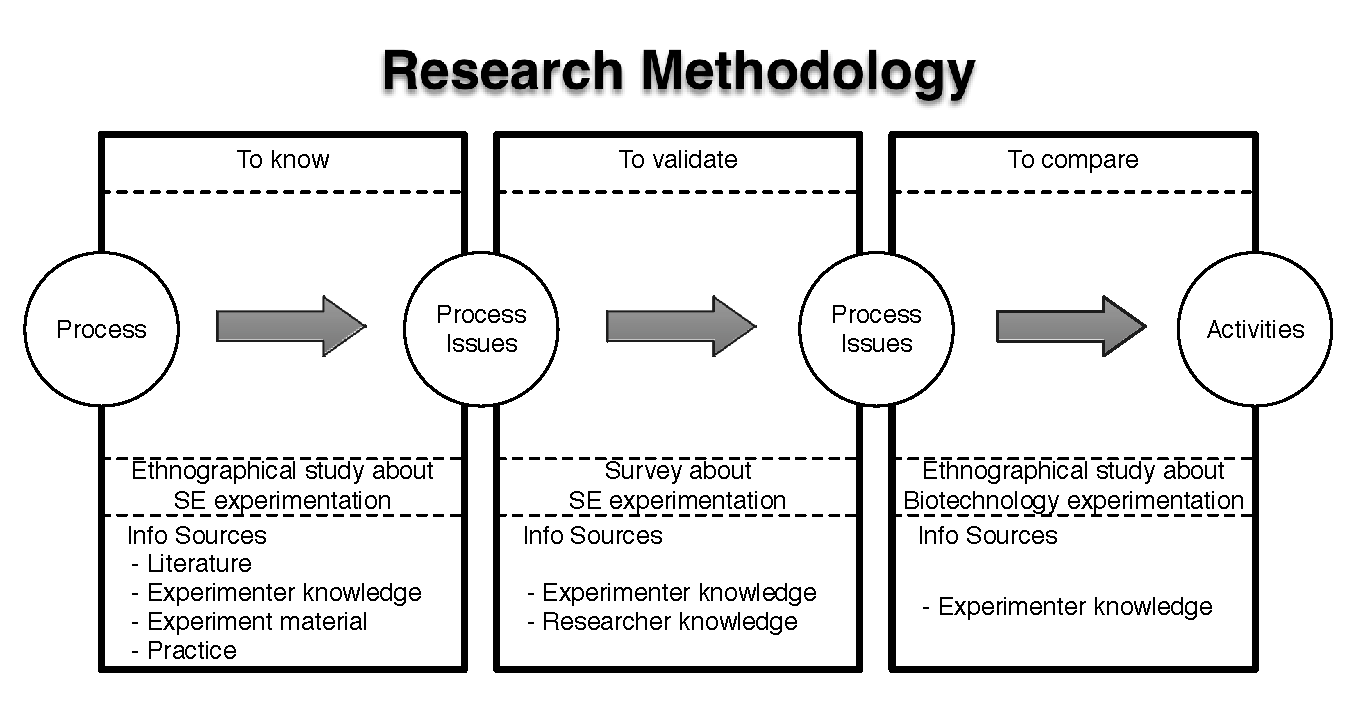
\includegraphics[width=12cm]{Images/Methodology}
	\caption{Research Methodology}
	\label{fig-research-methodology}
\end{figure*}

Cada una de las fases de investigaci�n fue guiada por un objetivo espec�fico, los cuales se listan a continuaci�n.

\begin{framed}%
%\textbf{SG2: How do researchers conduct SE experiments in practice?}
\textbf{SG1: To identify how researchers conduct SE experiments in practice into a specific research group}
\end{framed}

\begin{framed}%
%\textbf{SG1: How generalizable is the experimentation process performed into a specific SE research group?}
\textbf{SG2: To determine the generalizability of the experimentation process performed into a specific SE research group}
\end{framed}

\begin{framed}%
%\textbf{SG3: Does SE experimentation practice deviate from traditional disciplines?}
\textbf{SG3: To verify whether there is deviation of SE experimentation practice from traditional disciplines}
\end{framed}

In order to answer the research questions a mixed research methodology was applied. First, we conducted an ethnographical study to observe how a representative SE research group: Natalia Juristo's team (GrISE) at the Universidad Polit�cnica de Madrid (Spain) works. Since the results obtained from a unique research group are not necessarily generalizable, and the lack of depth in certain controversial aspects identified in GrISE, we performed a survey in order to strengthen our findings and extrapolating it to the ESE community. Finally, another ethnographical study was carried out in different representative research groups of Biotechnology at the Universidad de las Fuerzas Armadas ESPE (Ecuador). The aim of this second study was to compare SE experimentation in practice with that of another traditional discipline.

\subsection{Design of ethnographical studies}
Dar respuesta a RQ1 y RQ3 representa un gran desaf�o de investigaci�n, dado que supone el estudio de fuentes de informaci�n disponibles de un n�mero representativo de grupos de investigaci�n en ESE y en Biotecnolog�a, tal que se pueda conocer a detalle los retos que enfrenta el experimentador antes durante y despu�s de realizar las tareas de experimentaci�n en la pr�ctica. Todo esto, de la mano con el protocolo experimental descrito de forma te�rica en varias fuentes espec�ficas, tales como: textos, gu�as, manuales t�cnicos, reportes experimentales, entre otros.

Sin embargo, se torna muy complejo o casi imposible, realizar la investigaci�n en varias muestras del universo de grupos de investigaci�n de ambas disciplinas, dado el alto costo que esto representa (es decir, bloquear y controlar variables en los grupos, excesivo tiempo de investigaci�n en cada grupo, disponibilidad limitada de grupos afines para llevar a cabo la investigaci�n, disponibilidad limitada del tiempo de los experimentadores para con la investigaci�n, entre otros).

Esta situaci�n limita a que la investigaci�n sea llevada a cabo en un m�nimo n�mero de grupos de investigaci�n, lo que implica ciertos riesgos, dado que la validez de los resultados se ve amenazada. Para disminuir estos riesgos, creemos que los resultados deben responder a un riguroso proceso investigativo, los contextos de experimentaci�n seleccionados debe ser muy representativos en la poblaci�n bajo estudio y deben ser validados por otro medio los resultados obtenidos.

Visto desde esta perspectiva, se precisa aplicar una aproximaci�n emp�rica de observaci�n con alg�n tipo de interacci�n cuyo protocolo de investigaci�n se alinee con la naturaleza de la problem�tica identificada para garantizar la fiabilidad de los resultados obtenidos, enfatizar las caracter�sticas de la investigaci�n, su validez y significancia cient�fica \cite{sjoberg-2007-future-empical-methods}. Por lo tanto, los m�todos factibles a ser utilizados eran: etnograf�a, action research o case study.

En esta investigaci�n se necesitaba estudiar como se desarrolla un fen�meno (experimentaci�n) en su entorno natural (grupos de investigaci�n), por lo que realizamos an ethnographical study [REF].

\subsubsection{Context selection}
El criterio de selecci�n aplicado en los estudios etnogr�ficos parte de la premisa que un grupo de investigaci�n representativo representa una fuente fiable de informaci�n, lo que facilitar�a la tarea de aprendizaje respecto a la experimentaci�n. Por lo tanto, el criterio de selecci�n responde a las siguientes condiciones:

\begin{itemize}
\item{Ser un grupo de investigaci�n cuyos experimentadores tengan una consolidada experiencia den el �rea}

\item{Ser un grupo de investigaci�n cuyos experimentadores sean reconocidos en la comunidad cient�fica a trav�s de publicaciones de alto impacto, tales como libros, art�culos, manuales t�cnicos, entre otras.)}
\end{itemize}

%%%%%%%%%%%%%
%HASTA AQUI
%%%%%%%%%%%%%

Dadas las condiciones, los grupos de investigaci�n seleccionados son, por una parte, el Grupo GrISE perteneciente a la Escuela T�cnica Superior de Ingenieros Inform�ticos (ETSII) de la UPM de Espa�a y por otra parte, el �rea de Biotecnolog�a de Grupo de Investigaci�n en Modelos de Producci�n de Software (GrIMPSoft) perteneciente al Departamento de Ciencias de la Computaci�n (DECC) de la ESPE de Ecuador. Una descripci�n detallada de los grupos de investigaci�n seleccionados se realiza en las Secciones \ref{sec-execution-1} y \ref{sec-execution-2}, respectivamente.

\subsubsection{Data collection procedure(s)}\label{subsec-data-collection}
El proceso de recolecci�n de informaci�n que ser� aplicado consiste en un ciclo iterativo incremental de acciones realizadas sobre distintas fuentes de informaci�n (ver Figura \ref{fig-proceso-investigacion}), con el prop�sito de indagar sobre la experimentaci�n llevada a cabo en grupos de investigaci�n de distintas disciplinas.

\begin{figure}[htbp!]
	\centering
	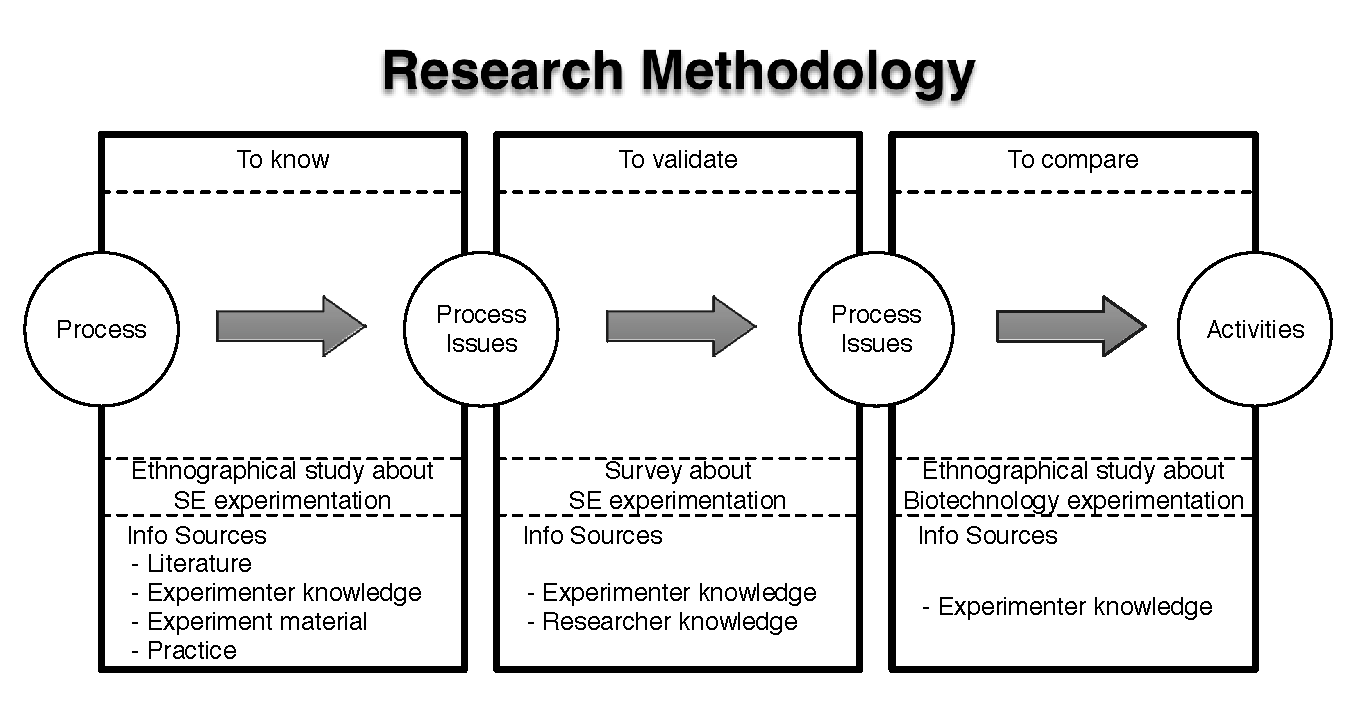
\includegraphics[width=3.5in]{Images/Methodology}
	\caption{Research Methodology}
	\centering
	\label{fig-research-methodology}
\end{figure}

Las fuentes generadoras de informaci�n corresponden espec�ficamente a aquellas que son accesibles y representativas dentro del grupo de investigaci�n bajo estudio. Para la presente investigaci�n se considera a la: Literatura com�n del grupo (general y espec�fica), material experimental del grupo (general y espec�fico) y conocimiento de los experimentadores del grupo (internos y externos).

El orden en el que el investigador tomar� contacto con las fuentes generadoras de informaci�n ser� aleatorio. La frecuencia de contacto con las fuentes depender� de la necesidad del investigador por obtener conocimiento; pero sobre todo, depender� de la disponibilidad de cada fuente. Es decir, mientras m�s disponible sea la fuente, el investigador podr� estar m�s tiempo en contacto con la misma. A continuaci�n se detalla la interacci�n que mantendr� el investigador con cada fuente.

\begin{itemize}
  \item En lo que respecta a la literatura com�n del grupo, el investigador tendr� acceso a la misma de forma inmediata y continua en el tiempo, a trav�s de distintos medios (por ejemplo: bibliotecas, bases digitales disponibles, versiones impresas disponibles, entre otras). La literatura representa una fuente de informaci�n muy importante, dado que proporcionar� la informaci�n referente al proceso de experimentaci�n, desde la perspectiva te�rica.
 
  \item El contacto con el material experimental m�s representativo y fiable propio del grupo de investigaci�n ser� inmediato y continuo en el tiempo, con la gu�a de los experimentadores. Sin embargo, para facilitar el proceso de revisi�n y aprendizaje de la informaci�n contenida en esta fuente, se precisar� un contacto previo con la literatura com�n del grupo. Eventualmente ser� preciso el estudio de material espec�fico para profundizar en una tem�tica particular. El material experimental representar� la evidencia de la experimentaci�n llevada a cabo en la pr�ctica por el grupo de investigaci�n.

  \item La obtenci�n del conocimiento de los experimentadores ser� planificada en funci�n de su disponibilidad de tiempo. Este proceso se realizar� desde un inicio, ya que se prev� una alta complejidad, considerando la aplicaci�n de distintas t�cnicas e instrumentos. Para el caso de los experimentadores externos, no ser� posible una planificaci�n espec�fica, dada la dificultad de un contacto directo; por lo tanto, en este punto mucho se depender� de la casualidad. El conocimiento obtenido de los experimentadores, representar� el proceso de experimentaci�n realizado en la practica dentro de los grupos de investigaci�n. 
\end{itemize}

Se prev� que el conocimiento obtenido de las fuentes indicadas se complementar�n entre si y servir� para determinar en qu� medida lo que que se encuentra expresado en la teor�a, corresponde a lo que efectivamente llevan a cabo los experimentadores en la pr�ctica dentro de los grupos de investigaci�n.

Para el proceso de extracci�n de la informaci�n se utilizar� una taxonom�a de t�cnicas de recolecci�n de informaci�n, categorizada de acuerdo al nivel de contacto con la fuente primaria de informaci�n, en este caso los experimentadores de cada entorno. La taxonom�a propone tres niveles de recolecci�n de informaci�n: Participaci�n directa con la fuente (nivel 1), participaci�n indirecta con la fuente (nivel 2) y estudio del material de trabajo (sin la participaci�n de la fuente) (nivel 3) \cite{Lethbridge-2005-studyingsoftwaredatacollection}.

El procedimiento para la recolecci�n de informaci�n de las fuentes indicadas, consiste en aplicar t�cnicas adecuadas dependiendo del tipo de fuente y de su disponibilidad. Por ejemplo, para extraer informaci�n de los experimentadores de un entorno de experimentaci�n se utilizar�n t�cnica t�cnicas tales como: entrevistas, grupos de discusi�n, entre otros (primer nivel). La adecuada aplicaci�n de las t�cnicas de recolecci�n de informaci�n estar� asociada a la utilizaci�n de diferentes instrumentos, algunos de los cuales se constituir�n como piezas fundamentales para recrear la informaci�n obtenida. Por ejemplo utilizaremos: videoc�maras, dispositivos de grabaci�n de audio, entre otros. M�s espec�ficamente, las t�cnicas de recolecci�n de informaci�n que se aplicar�n a las fuentes de informaci�n, se indican en la Tabla \ref{tbl-tecnica-fuente}.

\begin{table}
	\centering
	\caption{T�cnicas de recolecci�n por fuente de informaci�n}
	\label{tbl-tecnica-fuente}
	\begin{tabular}{|p{3cm}|p{3.7cm}|}
	\hline
	\textbf{Fuente} & \textbf{T�cnicas}\\
	\hline
	\multirow{7}{50 pt}{Conocimiento del grupo de investigaci�n} & Entrevistas\\
	\cline{2-2}
	& Grupos de discusi�n\\
	\cline{2-2}
	& Observaci�n participativa\\
	\cline{2-2}
	& Modelado de actividades\\
	\cline{2-2}
	& Sistemas instrumentales\\
	\cline{2-2}
	& Aprendizaje basado la experiencia\\
	\hline
	\multirow{1}{75 pt}{Literatura referente} & An�lisis de documentaci�n\\
	\hline
	\multirow{1}{75 pt}{Material experimental} & An�lisis de documentaci�n\\
	\hline
	\multirow{4}{50 pt}{Conocimiento de experimentadores externos} & Entrevistas\\
	\cline{2-2}
	& Grupos de discusi�n\\
	\cline{2-2}
	& Sistemas instrumentales\\
	&\\
	\hline
	\end{tabular}
\end{table}
 
Los inconvenientes presentados por el uso de las diferentes t�cnicas e instrumentos, ser�n minimizados gracias a su combinaci�n en cada iteraci�n. Por ejemplo, los vac�os del audio podr�n ser complementados por el video, las fotograf�as y los esbozos de los experimentadores y viceversa.

\subsubsection{Data analysis procedure(s)}
El procedimiento de an�lisis de datos tendr� un enfoque cualitativo y estar� asociado con la aplicaci�n de las t�cnicas de obtenci�n de informaci�n. Por lo tanto, este procedimiento tambi�n ser� de tipo iterativo incremental. El n�mero de iteraciones de an�lisis corresponder� al n�mero de iteraciones de recolecci�n de datos realizado con cada fuente. El procedimiento de an�lisis (ver Figura \ref{fig-proc-analisis}) se compone de dos actividades principales: (1) Verificaci�n de los datos y (2) Comparaci�n de los datos.

\begin{figure}[htbp!]
	\centering
	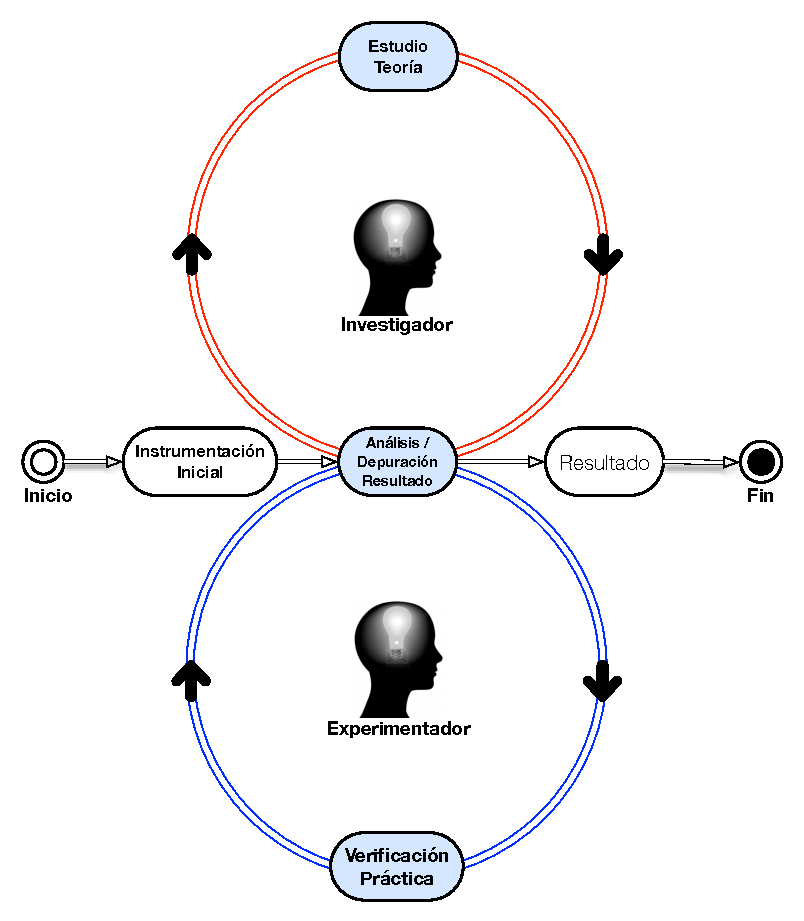
\includegraphics[width=2.5in]{Images/proceso-analisis}
	\caption{Proceso de An�lisis}
	\label{fig-proc-analisis}
\end{figure}

\begin{enumerate}[(a)]
\item \textbf{Verificaci�n de los datos: }Esta actividad tiene como objetivo verificar la validez de la informaci�n recolectada como insumo para el an�lisis, lo cual ser� realizado principalmente por los experimentadores del grupo. Durante las revisiones de las fuentes te�ricas, el investigador ir� adquiriendo paulatinamente conocimientos b�sicos de la experimentaci�n, lo cual le servir� para entender m�s f�cilmente los resultados obtenidos de la interacci�n con el conocimiento de los experimentadores. Estos resultados ser�n expresados de forma expl�cita en medios f�sicos o digitales y validados por el experimentador en cada iteraci�n hasta obtener el resultado final.
 
\item \textbf{Comparaci�n de los datos: } La comparaci�n de los datos obtenidos ser� realizada tanto por el investigador como por el experimentador, en una actividad de revisi�n cruzada, cada vez que hacen la verificaci�n de los datos en los resultados intermedios obtenidos. Por un lado el investigador hace la comparaci�n del resultado con su conocimiento adquirido de la revisi�n de otras fuentes de informaci�n; mientras que el experimentador compara el resultado con las actividades que efectivamente realiza en la pr�ctica. Una vez valida la informaci�n recabada el proceso de an�lisis concluye.
\end{enumerate}

\subsection{Survey of the experimentation process in SE}
y por otra parte, validaremos los hallazgos del proceso de etnograf�a en la comunidad de ESE a trav�s de un survey. Siguiendo los lineamientos propuestos por Runenson et al. \cite{case-study-in-SE-Runenson-2012} a continuaci�n detallamos: (1) El objetivo de la investigaci�n, (2) La descripci�n del procedimiento de selecci�n el caso, (3) el procedimiento de recolecci�n de datos y (4) Los procedimientos de validaci�n del estudio.

\section{Experimentation In Software Engineering}\label{sec-ESE-etnography}
El estudio fue realizado en el Grupo de Investigaci�n en Ingenier�a de Software Experimental (GrISE) de la Universidad Polit�cnica de Madrid (UPM). GrISE es un grupo que puede considerarse representativo de la comunidad de ESE. El origen del grupo data de finales de los 90s, cuando fue fundado por N. Juristo, una investigadora reconocida en IS por su temprano libro acerca de SE experimental \cite{Juristo2001} (con A. Moreno), adem�s de sus contribuciones posteriores. El grupo cuenta con otros investigadores de dilatada trayectoria, tales como Oscar Dieste y Sira Vegas. A lo largo de su historia, GrISE ha realizado varias familias de experimentos \cite{Basili1999-KnowledgeFamiliesExp}, en distintas tem�ticas: testing, requisitos y, m�s recientemente, test-driven development.

\subsection{First Approximation}\label{subsec-results-case1}
Los primeros contactos con el grupo de investigaci�n tuvieron lugar en 2012. Nuestra pretensi�n inicial era adquirir el conocimiento del grupo y volcarlo en modelos conceptuales, de una forma similar a la pr�ctica de la ingenier�a del conocimiento.

En un primer momento la tarea pareci� factible. Los miembros del GrISE hac�an continuas referencias a fuentes de consulta que ellos consideraban est�ndar, como por ejemplo el texto: \textit{Experimentation in Software Engineering} by Wohlin et al. \cite{Wohlin2000}; e igualmente a su material experimental, como por ejemplo a los: planteamientos de experimentos. Las primeras acciones de nuestra parte a llevar a cabo estaban claras: el estudio de la literatura preferida por el grupo y el estudio de su material experimental.

Sin embargo, pronto se evidenci� una barrera de entrada en el acceso al grupo: aunque el discurso del grupo era claramente general (e.g., nos hablaban de \textit{objetos experimentales} tal y como eran considerados en la literatura), su referente era eminentemente local (referido espec�ficamente a, material usado previamente por los miembros del grupo e.g., los programas usados en la familia de experimentos de testing). Esto dificultaba enormemente nuestra comprensi�n del modo en que el grupo llevaba a cabo su investigaci�n, confirm�ndose as� la necesidad de estudiar, adem�s de los textos est�ndar, tambi�n la literatura espec�fica del grupo.

\subsubsection{Review Of Preferred Literature}\label{subsubsec-study-literature}
Los miembros del GrISE se�alaron como fuentes b�sicas acerca de experimentaci�n en SE a los libros: \textit{Experimentation in Software Engineering} by Wohlin et al. \cite{Wohlin2000} and \textit{Basics of Software Engineering Experimentation} by Juristo et al. \cite{Juristo2001}. Ambos libros son probablemente los mejor conocidos \cite[p.~3]{Wohlin-2007-ESE-Teaching-Methods}, en parte tambi�n porque los textos de referencia son muy escasos. Tambi�n mencionaron de forma preferente los estudios: \textit{Building Knowledge Through Families of Experiments} \cite{Basili1999-KnowledgeFamiliesExp}, el cual parece una preferencia espec�fica del GrISE, dado su inter�s particular por realizar replicaciones experimentales; \textit{Experimentation in Software Engineering} \cite{Basili-1986-ESE}, el cual representa una de las primeras gu�as acerca de como llevar a cabo experimentos en SE; and \textit{Preliminary Guidelines for Empirical Research in Software Engineering} \cite{Kitchenham2002-GuideLinesESE}, las cuales son unas de las recomendaciones seminales acerca de como experimentar en SE.

Las fuentes anteriores fueron revisadas en profundidad por dos investigadores (E. Fonseca y E. Espinosa), quienes al momento en que se realiz� el estudio, contaban �nicamente con una formaci�n en ingenier�a tradicional y una especializaci�n en SE. Esta situaci�n les permiti� abstraer m�s f�cilmente los fundamentos de la SE experimental, que hasta ese entonces era un contexto totalmente desconocido para ellos; tal cual etn�grafos de principio del siglo XX visitando las tribus de �frica para entender sus costumbres y crear conocimiento de lo desconocido \cite{Aman-1978-africa-ethnography}.

En definitiva, los libros y art�culos estudiados propiciaron la adquisici�n del conocimiento espec�fico referido a conceptos tales como: Experimento, Replicaci�n, S�ntesis, Hip�tesis, Variables, Dise�o Experimental, entre otros; los cual permiti� comenzar la organizaci�n de dichos conceptos en un modelo conceptual preliminar, tal y como muestra la figura \ref{fig-conceptos-preliminar}.

\begin{figure}[htbp!]
	\centering
	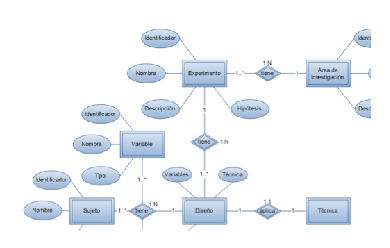
\includegraphics[width=3.2in]{images/Producto-Intermedio-Revision-Lit}
	\caption{Extracto del Modelo Conceptual Preliminar Abstra�do de la Experimentaci�n en GrISE}
	\label{fig-conceptos-preliminar}
\end{figure}

El primer aspecto que nos llam� la atenci�n fue la \textit{diversidad terminol�gica con que las distintas fuentes se refer�an a actividades similares del proceso experimental}. Para un observador sin conocimientos del �rea, la literatura parecer�a describir distintos tipos de experimentos, cada uno caracterizado por un proceso diferente. Una vez adquiridos los conocimientos b�sicos acerca de la materia, es inmediato percibir las similitudes, pero a�n as� no est� claro si los distintos autores est�n describiendo exactamente a las mismas actividades. Esto no ocurre solo a nivel de libros de texto, lo cual podr�a ser esperable, \textit{sino que tambi�n se extiende a otros materiales, tales como recomendaciones de reporte y art�culos}.

Podemos citar como ejemplos de la diversidad terminol�gica encontrada, a la denominaci�n heterog�nea utilizada por algunos autores para las fases del proceso de experimentaci�n en SE, tal como se indica a continuaci�n.

\begin{itemize}
	\item Juristo \& Moreno \cite{Juristo2001} proponen como fases del proceso a \textquotedblleft Objective Definition, Design, Execution and Analysis\textquotedblright.
	\item Wohlin et al. \cite{Wohlin2000} \textquotedblleft Experiment idea, Experiment scoping, Experiment planning, Experiment operation, Analysis \& interpretation, Presentation \& package and Experiment report\textquotedblright.
	\item Basili et al. \cite{Basili-1986-ESE} propose \textquotedblleft definition, planning, operation, and interpretation\textquotedblright.
\end{itemize}

Aunque los autores definen estas fases m�s en detalle en funci�n de las actividades que incluye cada una, la coincidencia en t�rminos y descripci�n difiere mucho de uno a otro autor.

Despu�s de buscar libros de texto complementarios a los indicados anteriormente, con la intenci�n de verificar si la diversidad terminol�gica era un problema general, o estaba circunscrito a las fuentes recomendadas, solo hemos localizado la nueva edici�n de Wohlin et al. \cite{Wohlin2012-Experimentation} sobre experimentaci�n y los libros especializados de Runeson et al. \cite{case-study-in-SE-Runenson-2012} y Kitchenham et al. \cite{Kitchenham-2015-Literature-Review-Book}. Preguntados a este respecto a los miembros del GrISE, nos se�alaron adicionalmente otras fuentes, tales como Box et al. \cite{Box2008} o Montgomery \cite{montgomery-2010-applied-statistics}, las cuales pertenecen al �rea de ingenier�a, pero no a la de experimentaci�n en SE. Por lo tanto, la \textit{carencia de textos sobre experimentaci�n en SE} es es otro aspecto noticeable. 

Esta situaci�n acrecent� nuestra convicci�n respecto a que la \textit{diversidad terminol�gica} pudiera ser todav�a mayor de la observada, incluyendo tambi�n una \textit{diversidad de aproximaciones y enfoques sobre la realizaci�n de experimentos}.

\subsubsection{Review of experimental material}\label{subsubsec-study-material}
El material experimental del grupo GrISE se compone fundamentalmente de: planteamientos de experimentos, dise�os experimentales, art�culos (e.g.: \cite{Juristo2012-EffectivenessWithinOutsideScopeExperiment,Juristo2006-SoftwareTestingTechniques,Juristo-2003-ESERNET}), instrumentos experimentales (e.g.: formularios de tareas experimentales, formularios de recogida de datos, gu�as), objetos experimentales (e.g.: programas con faltas sembradas, especificaciones de requisitos alteradas con anomal�as), raw data (e.g.: hojas de excel con datos de mediciones de tareas experimentales realizadas, bases de datos) y material de entrenamiento (e.g.: manuales t�cnicos \cite{Juristo2006-SoftwareTestingTechniques}, presentaciones).

El primer problema que nos encontramos fue el mismo acceso al material experimental, dado que \textit{no existe una pol�tica o herramienta para la gesti�n del material}. Un ejemplo paradigm�tico son los raw data. Encontramos raw data en distintos tipos de ficheros, correspondientes a distintas versiones, cuya ubicaci�n y formato son conocidos �nicamente por la persona que los gestiona. Lo mismo puede afirmarse, aunque en menor medida, de los restantes tipos de materiales (e.g.: instrumentos u objetos experimentales); con la excepci�n de las publicaciones, las cu�les son f�cilmente accesibles en las librer�as digitales.

Por lo tanto, fue preciso solicitar ayuda a los miembros del GrISE para acceder al material experimental, entender su estructura y la forma de gesti�n particular que utilizan. La revisi�n se realiz� de forma progresiva en funci�n de su antig�edad (i.e., primero revisamos lo m�s antiguo y luego lo m�s actual). Todas las fases de revisi�n fueron guiadas por el albacea de la informaci�n, cuyo relato sumado a la informaci�n obtenida del material revisado, nos permiti� descubrir que \textit{las actividades que generaron el material experimental han ido evolucionando y mejorando con el tiempo}. Por ejemplo, nos indicaron que los reportes experimentales, a pesar de haber sido aceptados en congresos y revistas de alto impacto, han ido perfeccion�ndose con el tiempo, sobre todo porque la exigencia de las revisiones se ha incrementado.

Otro aspecto que nos llam� la atenci�n en la revisi�n del material experimental, fue \textit{la extensi�n (entre 100 a 120 p�ginas) y complejidad del planteamiento de los experimentos}. Estos documentos se caracterizan por tener una \textit{descripci�n general de las actividades a ser realizadas en el experimento}, lo cual dificulta entender las particularidades que conlleva un experimento en la pr�ctica; por otra parte, \textit{no dan una gu�a sobre el orden de ejecuci�n de las actividades experimentales}. Por ejemplo, encontramos planteamientos de experimentos que inclu�an un dise�o experimental, mientras que otros no. Aquellos planteamientos con dise�o experimental, no especifican el tipo de dise�o que utilizan, solo indican su estructura y conformaci�n; adicionalmente, estos dise�os hac�an referencia a t�rminos totalmente diferentes a los identificados hasta el momento, y por ende dif�ciles de comprender, tales como: \textit{efecto del cansancio}, \textit{efecto del aprendizaje}, etc.

En contraste con la literatura revisada, encontramos definiciones similares con t�rminos diferentes, mismos t�rminos con definiciones diferentes, t�rminos diferentes con definiciones diferentes referidos al mismo concepto, y mismos t�rminos con definiciones similares. Con el prop�sito de mejorar el modelo conceptual que se ven�a estructurando, conservamos los conceptos que se manejan en el grupo, para el caso de los conceptos nuevos o con distinta terminolog�a, se opt� por utilizar los m�s comunes entre las fuentes consultadas. De acuerdo a estas consideraciones, se lleg� a elaborar el modelo conceptual que se muestra en la Figura \ref{fig-conceptos-final-revision-fuentes}.

\begin{figure}[htbp!]
	\centering
	
\includegraphics[width=3in]{images/Producto-Final-Revision-Lit}
	\caption{Estracto del Modelo Conceptual Abstra�do de la Experimentaci�n en GrISE}
	\label{fig-conceptos-final-revision-fuentes}
\end{figure}

Aunque en este punto cre�mos tener cierto nivel de conocimiento sobre la experimentaci�n en SE, las \textit{diferencias encontradas entre los materiales de las familias de experimentos revisadas}, acrecentaron nuestra \textit{incertidumbre sobre la fiabilidad de dichas fuentes}; por lo tanto, se torn� imperiosa la necesidad de revisar fuentes adicionales para intentar contrastar, incrementar y afianzar el conocimiento adquirido.

\subsection{Understanding The Experimental Process in SE}\label{subsec-second-aprox}
El estudio del material experimental propio del grupo constituy� sin duda una fuente de informaci�n fundamental para averiguar c�mo GrISE se enfrenta a la experimentaci�n, m�xime cuando refleja probablemente una gran cantidad de conocimiento t�cito del grupo, gestado en m�s de una d�cada de experimentaci�n. Sin embargo, el conocimiento contenido en el material experimental no era muy detallado, dado que \textit{no presentaba una gu�a clara de c�mo hacer un experimento}; adem�s, el estudio en este punto nos permiti� confirmar que efectivamente \textit{existe una diversidad de aproximaciones y enfoques sobre la realizaci�n de experimentos} en SE encontrados en las distintas familias de experimentos que el GrISE mantiene.

En este punto, vimos que la revisi�n de la literatura y del material experimental del GrISE ya no eran una opci�n para adentrarnos en los detalles m�s granulares de la experimentaci�n en SE; por lo tanto consideramos al aprendizaje en la pr�ctica como una opci�n, dado que posiblemente la ejercitaci�n con material experimental espec�fico, de la mano de la gu�a de los miembros del GrISE, constituir�a el camino a la familiarizaci�n de su formato, uso, e incluso verificaci�n de resultados; pero que especialmente, podr�a permitirnos la habituaci�n con actividades propias de la experimentaci�n, tales como: c�lculo de medidas a partir de la raw-data contenida en los materiales, formateo de la raw-data para an�lisis estad�stico, reproducci�n de resultados estad�sticos a partir de las mediciones, recreaci�n de gr�ficos y tablas estad�sticas a partir de las mediciones, etc. Por lo tanto, con la gu�a de los miembros del GrISE seleccionamos el material de un experimento particular, para intentar recrearlo y aprender de la pr�ctica en un entorno real.

\subsubsection{Review of Specific Experimental Material}\label{subsubsec-review-specific-material}
Este ejercicio consisti� en la revisi�n del material del experimento de t�cnicas de pruebas de software de Juristo et al. \cite{Juristo2012-EffectivenessWithinOutsideScopeExperiment}; a partir de la cual llevamos a cabo la replicaci�n \cite{Fonseca-2013-Replication-Efectiveness-In-Out}  en la Universidad de la Fuerzas Armadas ESPE, Sede Latacunga, de Ecuador.

\textit{Realizar en la pr�ctica una replicaci�n experimental sin duda permiti� entender de forma m�s did�ctica su proceso completo y las actividades inherentes}, e igualmente permiti� \textit{aclarar la concepci�n de la experimentaci�n obtenida en la revisi�n de la literatura referente y del material experimental del GrISE}. El hallazgo m�s importante de esta actividad fue \textit{comprobar la dificultad que representa llevar a cabo un experimento en la pr�ctica, m�s a�n al tratar de recrear fielmente un experimento ya realizado en un entorno diferente}, especialmente por la carencia de una gu�a detallada de actividades experimentales a realizar. Es preciso mencionar que la replicaci�n en sus fases iniciales cont� con la participaci�n directa de los investigadores que realizaron el experimento original, en este caso los mismos miembros del GrISE; cuyo aporte principal fue guiar el dise�o experimental, el uso del material experimental y dar los lineamientos espec�ficos para realizar la ejecuci�n y an�lisis del experimento.

No obstante, los resultados de la replicaci�n tuvieron diferencias marcadas con respecto al experimento original, incluso hubo errores en el an�lisis de resultados; posiblemente debido a factores propios del contexto donde se llev� a cabo la replicaci�n, o por falta de experiencia de quienes ejecutaron y analizaron los resultados de la replicaci�n, lo que al parecer indica que el conocimiento m�s granular sobre la ejecuci�n del experimento no fue abstra�do del todo para realizar la replicaci�n, o porque el conocimiento sobre la ejecuci�n y an�lisis de experimentos no fue abstra�do del todo de los lineamientos dados por los miembros del GrISE; confirm�ndose que \textit{no existe una gu�a clara y auto sustentable que permita realizar una replicaci�n literal del experimento original, siendo necesaria la presencia de los experimentadores originales en todo el proceso de la replicaci�n}.

Evaluando las actividades realizadas hasta el momento en la investigaci�n, encontramos que posiblemente el contenido de los textos de experimentaci�n revisados representen de forma expl�cita una parte del conocimiento de sus autores; sin embargo, comparando dicho contenido con los elementos del material experimental del GrISE, y con las actividades que no estaban indicadas en el material espec�fico revisado, y que nos fueron aclaradas para poder realizar la replicaci�n, vimos que las diferencias son muy marcadas, lo que muestra \textit{la generalidad de los textos, la falta de detalle del material experimental y la presencia de un conocimiento t�cito particular de cada investigador}; esto se confirma por la necesidad permanente de contar con la gu�a de los miembros del GrISE. Sin duda alguna las aproximaciones realizadas nos permitieron adquirir un conocimiento importante de la experimentaci�n en SE, pero era claro que el conocimiento m�s granular del proceso experimental lo ten�an los investigadores del GrISE. Por lo tanto, supimos con certeza el nuevo camino a seguir, intentar hacer expl�cito el conocimiento sobre experimentaci�n en SE de los miembros del GrISE.

\subsection{The Real Source Of Knowledge Regarding The Detailed Experimental Process in Software Engineering}\label{subsec-conocimiento-grupo}
Con el prop�sito de hacer expl�cito en un alto porcentaje el conocimiento granular de la experimentaci�n en SE que poseen los miembros del GrISE, lo cual, seg�n nos indicaron, no hab�a sido realizado anteriormente, cada miembro del GrISE paso a ser una fuente fundamental de informaci�n. Para alcanzar este objetivo, los miembros del GrISE nos concedieron paralelamente entrevistas personales y reuniones grupales de discusi�n.

\subsubsection{Interviews With GrISE Members}\label{subsubsec-interviews}
Las entrevistas a los miembros del GrISE se sustentaron en un cuestionario simple de preguntas abiertas orientadas a conocer a detalle las actividades que lleva a cabo cada miembro dentro del proceso experimental. El cuestionario se enfoc� en motivar en el entrevistado un relato libre y abierto sobre su rol en el proceso. En las primeras sesiones se afin� la t�cnica de abstracci�n de conocimiento para obtener el mayor detalle posible. Por ejemplo, se pas� de utilizar pluma y papel para tomar nota de las respuestas de los entrevistados, a grabaciones de audio y video; con lo cual, se agiliz� el proceso y sobre todo se pudo captar los detalles m�s granulares del entrevistado referidos a lo expresado, a los gestos, e incluso a los rasgos con los que algunos entrevistados esbozaban su relato ayudados de pluma y papel (por ejemplo ver Figura \ref{fig-proceso-exp-boseto}).

\begin{figure}[htbp!]
	\centering
	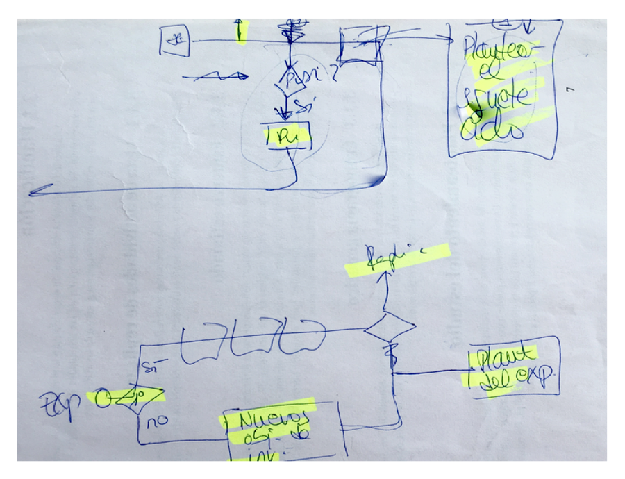
\includegraphics[width=3.2in]{images/Boseto-Proccess}
	\caption{Extracto de las actividades experimentales realizadas por los experimentadores del GrISE en boceto}
	\label{fig-proceso-exp-boseto}
\end{figure}

El conocimiento abstra�do en cada sesi�n de entrevistas fue validado con el entrevistado al inicio de la sesi�n posterior. El conocimiento abstra�do fue presentado al entrevistado en formato impreso compuesto en la mayor�a de los casos por texto, a diferencia de la informaci�n obtenida de la entrevista a la fundadora del GrISE, quien adicion� en su relato un boceto sobre las actividades del proceso experimental, el cual fue recreado con herramientas inform�ticas (ver Figura \ref{fig-proceso-exp-boseto}), lo que mostr� que \textit{los experimentadores de mayor experiencia tienen un conocimiento m�s amplio y detallado sobre las actividades que se llevan a cabo en la experimentaci�n en SE}.

El proceso de entrevistas realizado permiti� depurar los resultados intermedios del proceso experimental, tanto en relato escrito como gr�fico (por ejemplo ver Figura \ref{fig-proceso-draft}) y termin� tanto en cuanto el entrevistado indic� que su relato sobre las actividades que realiza en el proceso experimental hab�a concluido y estaba de acuerdo con el resultado final obtenido (por ejemplo ver Figura \ref{fig-proceso-exp}). Una situaci�n particular que nos llam� la atenci�n fue que \textit{el detalle de actividades obtenido en el flujograma del proceso experimental de, por ejemplo, la Figura \ref{fig-proceso-exp}, indica que los textos sobre experimentaci�n en SE existentes y el material experimental del grupo est�n lejos de mostrar el trabajo real que implica la experimentaci�n en la pr�ctica de principio a fin.}

\begin{figure}[htbp!]
	\centering
	\includegraphics[width=3.2in]{images/Proccess-Draft}
	\caption{Extracto de las actividades experimentales realizadas por los experimentadores del GrISE (versi�n intermedia)}
	\label{fig-proceso-draft}
\end{figure}

\begin{figure}[htbp!]
	\centering
	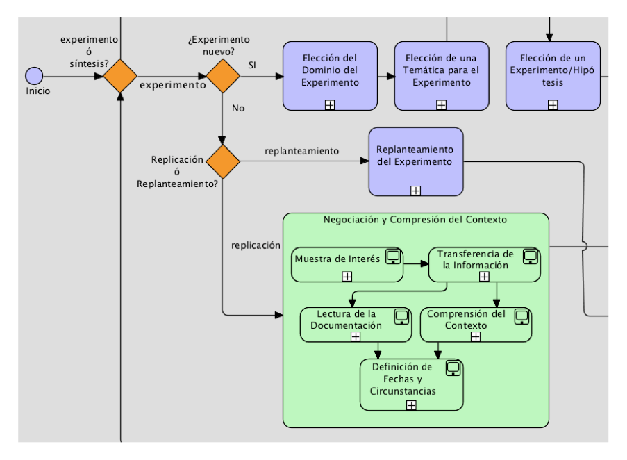
\includegraphics[width=3.2in]{images/Proccess}
	\caption{Extracto de las actividades experimentales de SE realizadas por los experimentadores del GrISE (versi�n final)}
	\label{fig-proceso-exp}
\end{figure}

Por otra parte, el proceso de entrevistas mostr� que \textit{las actividades realizadas por los experimentadores entrevistados difieren de un experimentador a otro, de hecho ning�n experimentador entrevistado lleva a cabo todas las actividades identificadas de la experimentaci�n en SE.} Ante esto fueron consultados los miembros del GrISE, quienes indicaron que \textit{no existe una definici�n explicita para el grupo actividades que realiza cada experimentador}; de hecho, ese momento acordaron identificar 3 grupos de actividades espec�ficas que realizaban los miembros del GrISE y los denominaron como los roles: Research Manager (RM), Experiment Manager (EM) and Senior Experimenter (SE), los cuales en t�rminos generales se encargan de: \textit{planificar la ejecuci�n del experimento, ser el albacea de la informaci�n y gestionar la log�stica de la experimentaci�n}, respectivamente.

En este punto, nos llam� la atenci�n que entre los roles identificados \textit{existen actividades experimentales que son ejecutadas por duplicado en una misma instancia experimental. Como por ejemplo: La gesti�n de la replicaci�n experimental la realizan el RM y el EM, el planteamiento del experimento lo realizan el SE y el RM}. Esto ratifica la diversidad de criterios existente dentro del GrISE, de la mano de la diversidad terminol�gica utilizada para las actividades que realizan. Esta situaci�n alert� a los miembros del GrISE y propiciaron reuniones a modo de grupos de discusi�n sobre esta tem�tica, puntualmente para intentar formalizar la terminol�gica utilizada en la experimentaci�n.

\subsubsection{Formalizing de Experimental Terminology in SE}\label{subsubsec-focus-groups}
El modelo conceptual estructurado en base a la revisi�n de la literatura preferida y del material experimental del GrISE (ver Figura \ref{fig-conceptos-final-revision-fuentes}), sirvi� como punto de partida de la discusi�n sobre la diversidad terminol�gica y operativa de la experimentaci�n en SE identificada en las diferentes fuentes revisadas hasta el momento.



La t�cnica de Focus Groups se apoy� en las mismas t�cnicas e instrumentaci�n de la entrevista, con el prop�sito de que los miembros del equipo de trabajo puedan esbozar y participar en el modelado conceptual de la experimentaci�n en SE, el investigador participe activamente en el debate sobre las propuestas de los experimentadores y el investigador cubra inquietudes menores con el experimentador sin tener necesariamente contacto personal.

El proceso de Focus Groups sobre la terminolog�a manejada en la experimentaci�n en SE fue c�clico. Se parti� de un boceto creado en consenso por los experimentadores en la pizarra (ver Figura \ref{fig-conceptos-draft}), luego de lo cual se realizaron varias sesiones de focus groups. En cada instancia de Focus Groups se gener� un producto intermedi�, el cual fue validado por el grupo en la siguiente sesi�n, hasta obtener el producto final (ver Figura \ref{fig-conceptos-exp-boseto}).

\begin{figure}[htbp!]
	\centering
	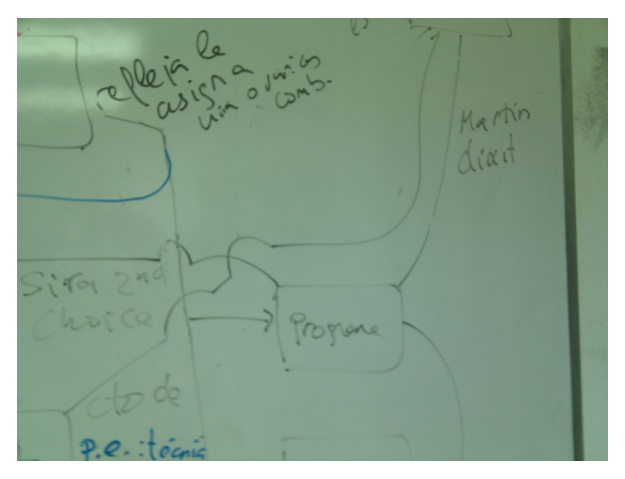
\includegraphics[width=3in]{images/Concept-Draft}
	\caption{Extracto del Modelo Conceptual de la Experimentaci�n en GrISE en Boceto}
	\label{fig-conceptos-draft}
\end{figure}

\begin{figure}[htbp!]
	\centering
	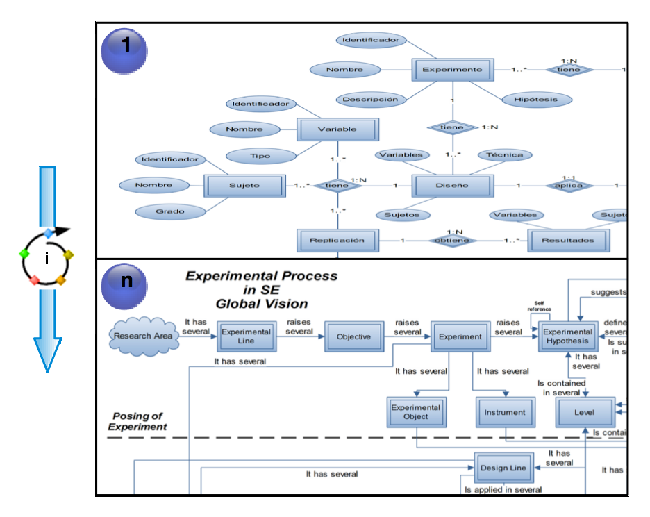
\includegraphics[width=3in]{images/Boseto-Concepts}
	\caption{Extracto del Modelo Conceptual de la Experimentaci�n en GrISE (versi�n final)}
	\label{fig-conceptos-exp-boseto}
\end{figure}

El producto obtenido de este primer proceso de Focus Groups fue un modelo conceptual gen�rico de la experimentaci�n en SE (ver Figura \ref{fig-conceptos-exp-boseto}), el cual no fue consensuado por el grupo. Por lo tanto, se llev� a cabo otro proceso de focus groups, con la particularidad de que cada experimentador indic� �nicamente los conceptos que maneja a trav�s de las actividades que efectivamente realiza en una instancia experimental. Este nuevo ciclo de Focus Groups gener� tres modelos conceptuales, los cuales se muestran en la Figura \ref{fig-conceptos-exp}. Es preciso mencionar que estos modelos responden a los tres roles identificados durante el proceso de entrevistas.

\begin{figure}[htbp!]
	\centering
	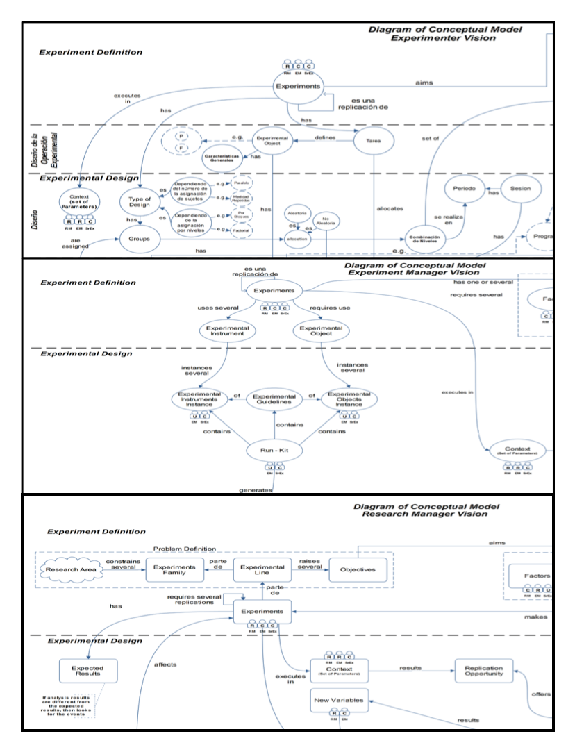
\includegraphics[width=3in]{Images/Concepts}
	\caption{Extracto de los Modelo Conceptuales}
	\label{fig-conceptos-exp}
\end{figure}

Los hallazgos identificados en base a los resultados obtenidos son:

\begin{itemize}
	\item El nivel de detalle conceptual del experimentador que se encarga de la ejecuci�n misma de un experimento es muy alto.
	
	\item Se evidenci� la diversidad terminol�gica entre experimentadores que realizan actividades similares en una instancia experimental en SE.
	
	\item Se evidenci� discrepancia conceptual sobre las actividades de experimentaci�n en SE entre experimentadores.
	
	\item Se confirm� que los conceptos manejados por los experimentadores en SE obedecen a las actividades espec�ficas que realizan en una instancia experimental.
	
	\item Se evidenci� la existencia de roles o perfiles de experimentadores: Experimentadores que custodian el material experimental del grupo, experimentadores que ejecutan en la pr�ctica la experimentaci�n y experimentadores que gestionan con el medio externo los nuevos experimentos y su factibilidad.
\end{itemize}

\subsection{Conclusions Around Software Engineering Experimentation Process}
Los resultados de la investigaci�n constituyen una visi�n expl�cita de la experimentaci�n en SE dentro de un grupo de investigaci�n representativo de la comunidad de ingenier�a de software emp�rica, incluso para los mismos experimentadores que ve�an por primera vez plasmado de forma expl�cita en medios accesibles el modelo de la experimentaci�n en SE. M�s espec�ficamente, las conclusiones obtenidas a partir de esta investigaci�n son:

\begin{enumerate}[(a)]
\item La generalidad de los textos existentes y la diversidad estructural de los reportes experimentales en la comunidad de ingenier�a de software emp�rica no representan una gu�a efectiva para llevar a cabo una instancia experimental en la pr�ctica.
 
\item La falta de formalizaci�n de los reportes experimentales impide realizar una lectura compresiva est�ndar, ya que para cada reporte es preciso descubrir su particularidad al momento de reportar.

\item El uso de formatos distintos en los reportes impide identificar de forma eficiente las actividades llevadas a cabo en una instancia de experimentaci�n en SE.

\item El formato de los archivos que contienen los datos experimentales de las instancias experimentales, no son est�ndar, por lo que es imposible que una persona ajena al grupo de trabajo entienda los conceptos, entidades y acr�nimos utilizados.

\item Se pudo percibir la posibilidad de que la existencia de mecanismos automatizados que guarden el v�nculo entre los experimentos y sus elementos (materiales, raw-data, dise�o, etc.), podr�an ayudar a los experimentadores a no cometer errores, dado el alto n�mero de actividades que deben cubrir.

\item Una comunicaci�n m�s cercana con los experimentadores, permiti� encontrar detalles que generalmente no se reflejan en los reportes experimentales y que ayudaron a entender algunos resultados, conclusiones de los reportes experimentales y llevar a cabo una replicaci�n experimental.

\item Durante las entrevistas personales mantenidas con los experimentadores se evidenci� un tipo de informaci�n impl�cita de los experimentos, la cual no es registrada en ning�n medio. Este tipo de informaci�n posiblemente proviene de la dimensi�n t�cita del conocimiento.

\item La deficiencia en la gesti�n de la informaci�n dentro del GrISE podr�a deberse a la diversidad operativa de los experimentadores, lo que dificulta el intercambio de informaci�n.
\end{enumerate}

\section{The Experimentation in Biotechnology}\label{sec-case-study-2}
La formalidad del proceso experimental de las disciplinas tradicionales nos motiv� a indagar los detalles de las actividades que realizan, para validar la problem�tica identificada en la ESE. La investigaci�n se llev� a acabo en la Universidad de las Fuerzas Armadas ESPE (Ecuador) en la Carrera de Ingenier�a en Biotecnolog�a.

La experimentaci�n en Biotecnolog�a es compleja dado el n�mero de actividades involucradas, la extensa variedad de insumos y los instrumentos que se precisan (dependiendo del �rea de investigaci�n) \cite{Kumar-2014-design-experiment-bioprocessing}. Sin embargo, nuevas propuestas sobre dise�o de experimentos (e.g.: dise�os basados en el enfoque), ofrecen una alternativa de formalizaci�n del proceso experimental \cite{Kumar-2014-design-experiment-bioprocessing}, lo que precisamente fue indagado en la presente investigaci�n.

\subsection{Context}\label{subsec-context-case-study-2}
Para este estudio se consider� a distintos grupos de investigaci�n de la Carrera de Biotecnolog�a. A pesar de que desconocemos el grado de representatividad de los grupos de investigaci�n objeto de estudio, creemos que es alto, dado el nivel de publicaciones realizadas (por citar un par de ejemplos: \cite{Vizuete-2016-green-Synthesis,Villarreal-2016-Effect-Arbuscular,Kumar-2016-In-Vitro-Evaluation}).

De acuerdo al criterio de selecci�n indicado en la Secci�n \ref{sec-methology}, estudiamos las actividades experimentales realizadas por grupos de investigaci�n en las �reas de Biotecnolog�a Humana, Biotecnolog�a Ambiental y Biotecnolog�a Vegetal. Estos grupos est�n liderados por un investigador (generalmente el director de un proyecto o jefe de un laboratorio), e incluyen estudiantes de doctorado y master. Adicionalmente, los grupos mantienen convenios con universidades de distintos pa�ses y disponen de una vasta cantidad de datos experimentales locales y/o p�blicos.

\subsection{Results}\label{subsec-results-case-study-2}
Los resultados obtenidos respecto al estado de la pr�ctica de la experimentaci�n en Biotecnolog�a son descritos en esta secci�n. Las fuentes de informaci�n estudiadas fueron: (1) Literatura referente a los grupos y (2) Conocimiento de los experimentadores.

En este estudio de caso no se realiz� una revisi�n del material experimental existente en los grupos de investigaci�n, dado que era muy espec�fico debido a la naturaleza propia de cada tem�tica de investigaci�n. Es preciso mencionar que los experimentadores indicaron que los datos obtenidos en las instancias experimentales son utilizados hasta su reporte, luego de lo cual son almacenados en repositorios de informaci�n experimental locales o p�blicos para futuros an�lisis. 

\subsubsection{Review of concerning literature}\label{subsubsec-study-literature-case-study-2}
Esta fuente de informaci�n corresponde a textos cient�ficos del �rea de Biotecnolog�a, publicaciones propias de los grupos objeto de estudio y a las denominadas libretas de laboratorio. Dichas fuentes de informaci�n fueron revisadas de forma exhaustiva, lo que permiti� obtener conocimiento y argumentos para generar debates en grupos de discusi�n; as� como, para evaluar y modificar modelos conceptuales y de proceso esbozados en distintas entrevistas. Adem�s, el estudio de las publicaciones de estos grupos permiti� indagar sobre el estado de la pr�ctica de la Biotecnolog�a.

Para realizar el estudio de literatura se utiliz� la t�cnica de an�lisis de documentaci�n (tercer nivel), con el apoyo de software especializado en gesti�n documental, tecnolog�as de la informaci�n, entre otros. Este estudio permiti� abstraer los aspectos fundamentales de la experimentaci�n en Biotecnolog�a, tales como las actividades realizadas y los artefactos utilizados.

The review of the concerning literature obtained the following results:
\begin{itemize}
  \item El proceso de experimentaci�n en Biotecnolog�a est� descrito de forma general en los textos cient�ficos revisados. Por ejemplo en el libro Biotechnology Fundamentals de Khan \cite{Khan-2012-Biotechnology-Fundamentals}.
  
  \item Los textos, gu�as, reportes, etc. sobre experimentaci�n en Biotecnolog�a son numerosos, pero espec�ficos por tem�ticas de investigaci�n. Por ejemplo, en la Biotecnolog�a Agr�cola el libro de Solaiman et al. \cite{Solaiman-2014-Mycorrhizal} describe el uso de microorganismos que se aplican a cultivos para el uso sustentable del suelo. En la Biotecnolog�a Vegetal el libro de Bahadur et al. \cite{Bahadur-2015-Plant-Biotechnology} estudia todas las �micas de \textit{Arabidopsis thaliana} como modelo para el mejoramiento gen�tico de otras plantas.
  
  \item Se encontr� formalidad (terminol�gica y operativa) del proceso de experimentaci�n de Biotecnolog�a en fuentes biogr�ficas de tem�ticas espec�ficas. Por ejemplo, el handbook de Walker et al. \cite{Walker-2008-Handbook-Biomethods} y el libro de Ausubel et al. \cite{Ausubel-2003-Molecular-Biology} denotan mucha similaridad en el protocolo experimental utilizado para el estudio de �cidos nucleicos.
  
  \item Se encontr� diversidad terminol�gica y operativa entre fuentes de distintas tem�ticas. %Por ejemplo en el libro de Villacr�s et al. \cite{Villacres-2015-Banco-HMA} se menciona
  
  \item Los reportes experimentales de los grupos de investigaci�n estudiados son similares en formato y centran su discurso en los resultados generales de cada ensayo (experimento), los cuales se basan en la comparaci�n de  resultados de tratamientos individuales.
  
  \item Encontramos indicios de que las actividades de experimentaci�n realizadas en Biotecnolog�a son el fundamento de la estructura de los reportes experimentales.
  
  \item El estudio de textos cient�ficos permiti� la adquisici�n de un conocimiento general sobre la experimentaci�n en Biotecnolog�a; el cual, en adici�n al conocimiento obtenido de otras fuentes, fue hecho expl�cito en un modelo conceptual b�sico (ver Figura \ref{fig-modelo-conc-inicial}) que sirvi� como insumo inicial en el proceso de grupos de discusi�n.
\end{itemize}

\begin{figure}[htbp!]
	\centering
	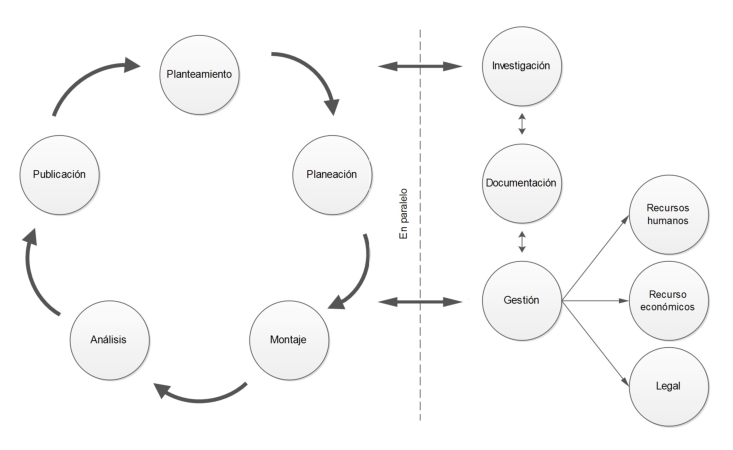
\includegraphics[width=3.2in]{Images/Modelo-Conceptual-Inicial}
	\caption{Modelo Conceptual Inicial}
	\label{fig-modelo-conc-inicial}
\end{figure}

\subsubsection{Obtenci�n de Conocimiento de los Grupos de Investigaci�n}\label{subsubsec-conocimiento-grupos}
El conocimiento obtenido de los grupos de investigaci�n signific� el insumo m�s representativo de esta investigaci�n. Esta actividad permiti� hacer expl�cito el conocimiento de los experimentadores de Biotecnolog�a. 

La obtenci�n del conocimiento de los experimentadores se sustent� principalmente en dos t�cnicas: (1) Entrevistas sobre las actividades experimentales que realizan, y (2) Focus Groups sobre los conceptos que manejan.

\textbf{Entrevistas sobre las actividades experimentales de Biotecnolog�a}\\
El proceso de entrevistas a los experimentadores de Biotecnolog�a se llev� a cabo en varias sesiones con cada experimentador. Por cada sesi�n se gener� un reporte que fue validado por el experimentador en la sesi�n siguiente, hasta obtener un manuscrito que sintetiza detalladamente las actividades experimentales que realiza.

De forma paralela a las entrevistas, algunos experimentadores realizaron esbozos en papel o en la pizarra de las actividades que realizan en el proceso experimental, como se indica en la Figura \ref{fig-proc-exp-esbozo}. Estos esbozos fueron sintetizados en un �nico modelo, que fue digitalizado utilizando software especializado. En cada sesi�n fue validado el modelo por los experimentadores (ver Figura \ref{fig-proceso-exp-intermedio}), hasta obtener un modelo final (ver Figura \ref{fig-proceso-exp-final}).

\begin{figure}[htbp!]
	\centering
	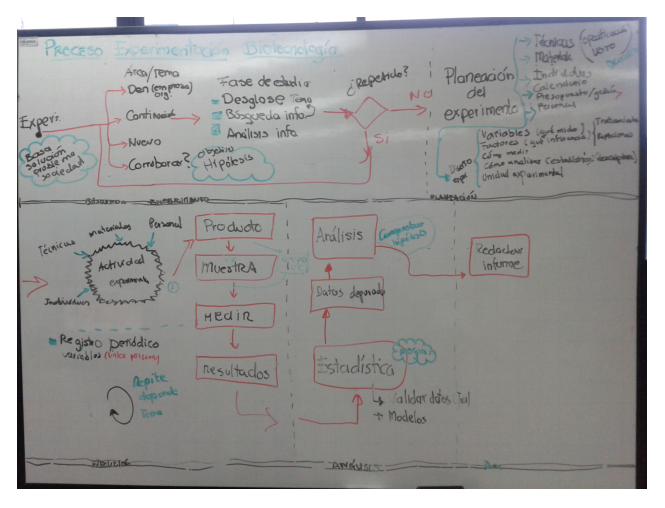
\includegraphics[width=3.2in]{Images/Outline-Process}
	\caption{Ejemplo de Esbozo de las Actividades Experimentales de Biotecnolog�a}
	\label{fig-proc-exp-esbozo}
\end{figure}

\begin{figure}[htbp!]
	\centering
	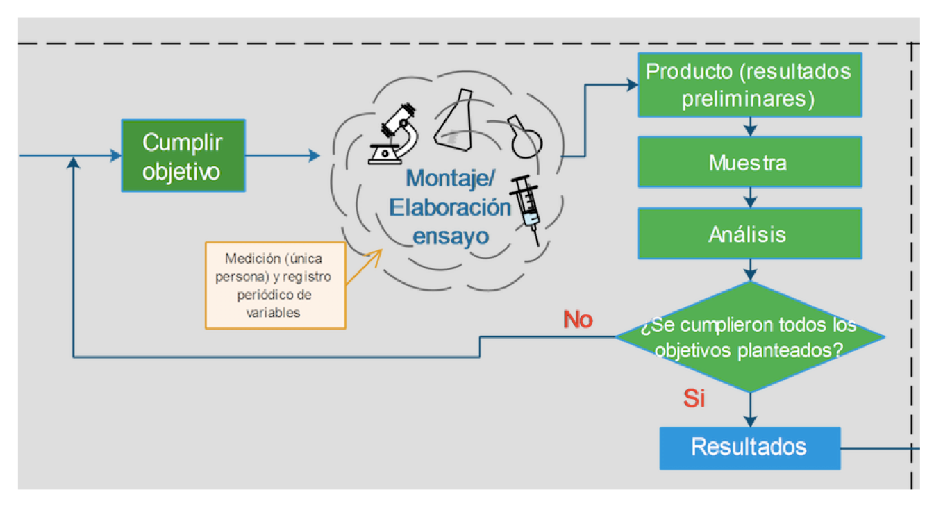
\includegraphics[width=3.2in]{Images/Intermediate-Process}
	\caption{Extracto Inicial del Proceso Experimental de Biotecnolog�a}
	\label{fig-proceso-exp-intermedio}
\end{figure}

\begin{figure}[htbp!]
	\centering
	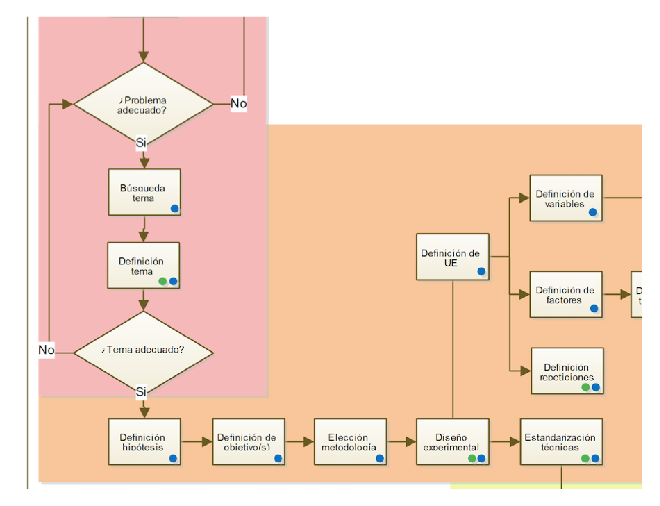
\includegraphics[width=3.2in]{Images/Final-Process}
	\caption{Extracto del Proceso Experimental de Biotecnolog�a}
	\label{fig-proceso-exp-final}
\end{figure}

Como complemento a las entrevistas, se utilizaron t�cnicas de modelado de conceptos, observaci�n participativa y sistemas instrumentales, con el prop�sito de recrear los esbozos de forma fidedigna en herramientas inform�ticas, coadyuvar ideas generadas en la entrevista y recibir un feedback complementario a trav�s de medios tecnol�gicos, respectivamente.

Para la aplicaci�n de las t�cnicas mencionadas se utilizaron mecanismos tecnol�gicos que capturan en video, audio y fotograf�as los detalles de las entrevistas; as� como tambi�n, herramientas inform�ticas para hacer expl�cito el conocimiento adquirido tanto en texto como en gr�ficos.

Los resultado obtenidos a partir de las entrevistas son: 

\begin{itemize}
  \item El modelo de procesos obtenido sugiere que el protocolo experimental de Biotecnolog�a es formal y bastante detallado.
  \item Cada experimentador lleva a cabo actividades definidas dentro del proceso de experimentaci�n en Biotecnolog�a. El conjunto de actividades realizadas por cada experimentador cumple un rol con una denominaci�n especifica, por ejemplo el \textit{Biometrista} se encarga del an�lisis de datos.
  \item No existe solapamiento de actividades en el proceso de experimentaci�n, dado que cada experimentador cumple un rol.
\end{itemize}

\textbf{Focus Groups sobre los conceptos manejados en el proceso de experimentaci�n en Biotecnolog�a}\\
El Focus Group para recabar la terminolog�a utilizada en el proceso de experimentaci�n en Biotecnolog�a fue realizado en varias sesiones. El proceso inici� con el debate sobre el modelo conceptual resultante de la review of the concerning literature (ver Figura \ref{fig-modelo-conc-inicial}). A continuaci�n, se realizaron varias sesiones con los experimentadores. De cada sesi�n se obtuvo un producto intermedi� (ver Figura \ref{fig-concepts-draft-bio}), el cual fue validado por el grupo en la siguiente instancia, hasta obtener un producto final (ver Figura \ref{fig-concepts-final-bio}).

\begin{figure}[htbp!]
	\centering
	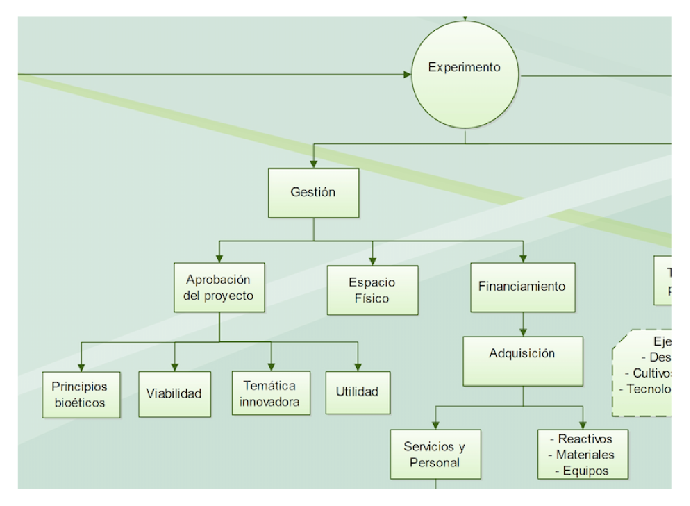
\includegraphics[width=3in]{Images/Concepts-Draft-Bio}
	\caption{Extracto del Modelo Conceptual Inicial de Biotecnolog�a}
	\label{fig-concepts-draft-bio}
\end{figure}

\begin{figure}[htbp!]
	\centering
	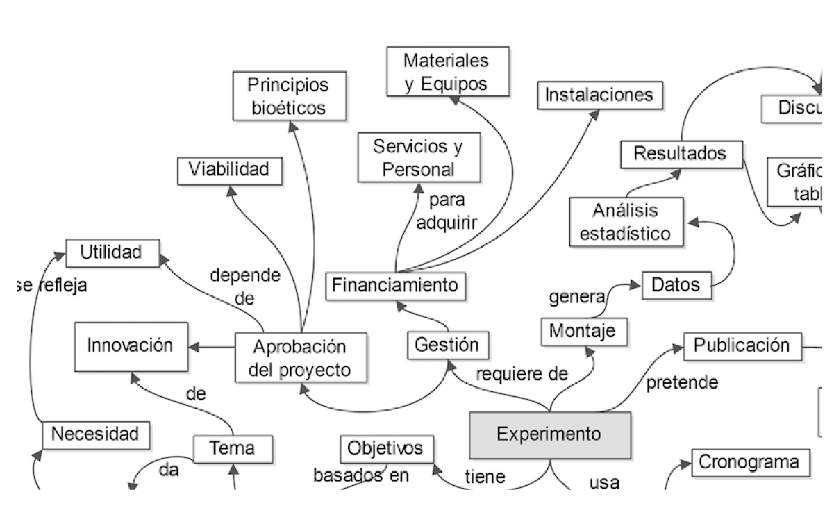
\includegraphics[width=3in]{Images/Concepts-Final-Bio}
	\caption{Extracto del Modelo Conceptual de Biotecnolog�a}
	\label{fig-concepts-final-bio}
\end{figure}

Como complemento al Focus Group se aplicaron t�cnicas de modelado de conceptos, observaci�n participativa y sistemas instrumentales; con el prop�sito de esbozar el modelo, participar activamente en el modelado conceptual, y sustentar dudas menores con cada experimentador, respectivamente. Para estas t�cnicas se utilizaron los mismos instrumentos y herramientas que en las entrevistas.

Los resultado obtenidos a partir del Focus Group son:

\begin{itemize}
	\item La cantidad de conceptos que intervienen en el proceso de experimentaci�n en Biotecnolog�a es alta.
	\item Se constat� que los experimentadores de un mismo grupo de investigaci�n en Biotecnolog�a utilizan una terminolog�a com�n para comunicarse.
	\item Se observ� que los conceptos manejados por los experimentadores en Biotecnolog�a corresponden a las actividades espec�ficas del rol que cumplen en cada proceso experimental.
\end{itemize}

\subsection{Conclusions}
\begin{enumerate}[(a)]
\item Los textos gen�ricos de Biotecnolog�a no representan un gu�a efectiva para llevar a cabo experimentos en la pr�ctica en �reas espec�ficas.

\item La formalidad de los reportes experimentales de �reas espec�ficas de la Biotecnolog�a permiten replicar sin mayor complicaci�n los estudios realizados.

\item La formalidad en los reportes permite identificar f�cilmente las actividades llevadas a cabo en un proceso experimental.

\item El formato de los contenedores de datos experimentales es est�ndar (hojas excel o repositorios), lo que facilita el acceso y utilizaci�n a otros grupos que investigan sobre la misma tem�tica.

\item El uso de mecanismos automatizados que guarden el v�nculo entre los experimentos y sus elementos (materiales, raw-data, dise�o, etc.) es fundamental y usual en Biotecnolog�a, ya que ayuda a los experimentadores, entre otras cosas, a gestionar f�cilmente los datos experimentales.

\item Los detalles de los reportes experimentales de Biotecnolog�a son muy expl�citos, tal es as� que sin ser conocedores o expertos en el �rea, se puede entender claramente sus resultados, conclusiones y discusi�n.

\item La efectividad de la gesti�n de la informaci�n dentro de los grupos estudiados podr�a deberse a la formalidad operativa de su proceso; lo que facilita el intercambio de informaci�n.
\end{enumerate}

\input{tex/comparison}

\section{Survey on Experimentation in Software Engineering}\label{sec-survey}
En base a los resultados del estudio entnogr�fico de la experimentaci�n en SE (Secci�n \ref{sec-methology}), nos preguntamos si la praxis del grupo de investigaci�n seleccionado coincide con la de la comunidad de ESE. M�s espec�ficamente, nos preguntamos si:

\begin{itemize}
	\item �Se ha formado la comunidad de ESE de modo similar al grupo de investigaci�n estudiado?
	\item �Son comunes los materiales de aprendizaje utilizados por la comunidad ESE y el grupo de investigaci�n estudiado?
	\item �Existe diversidad terminol�gica sobre experimentaci�n en la comunidad de ESE?
	\item �Existe diversidad operativa?
	\item �Existen roles asociados a la realizaci�n de tareas particulares?
\end{itemize}

El cuestionario planteado en el survey justamente se enfoc� en dar respuesta a estas interrogantes. La encuesta fue promovida durante the 2016 Empirical Software Engineering International Week (ESEIW) realizada en Ciudad Real (Spain). Este evento re�ne a los investigadores m�s emblem�ticos de la comunidad de ESE, y representa por lo tanto una poblaci�n adecuada para realizar el survey. La encuesta fue instrumentada a trav�s de Google Forms. 27 investigadores de diferentes partes del mundo participaron en el survey, lo que teniendo en consideraci�n los asistentes a la conferencia (112 personas, seg�n nos inform� la Conference Chair) supone un 24\% de response rate. Los investigadores de USA (4), Brazil (4) e Italia (3) son los que m�s representaci�n tuvieron (ver Fig. \ref{fig-nationality-respondents}), aunque obtuvimos respuestas de investigadores de 15 pa�ses.

\begin{figure}[htbp!]
	\centering
	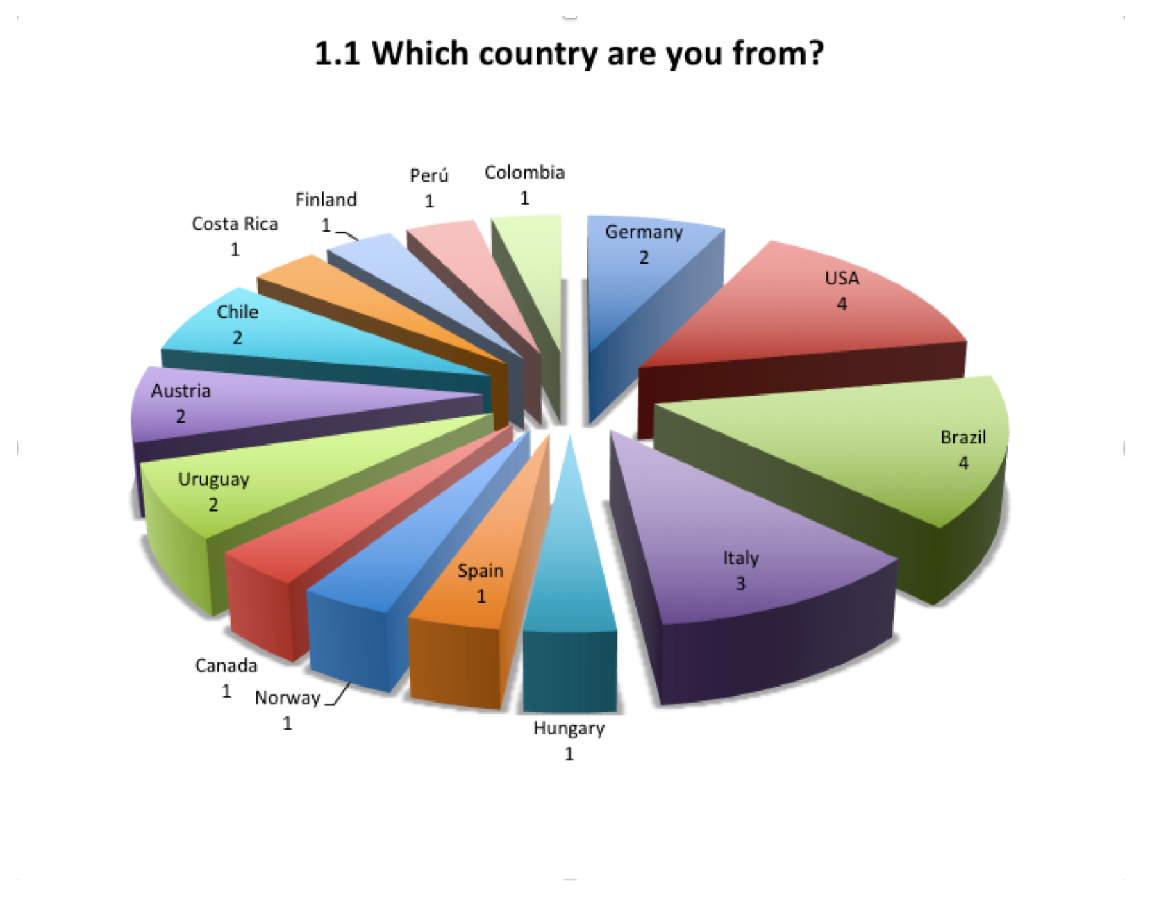
\includegraphics[width=3.4in]{Images/Nationality-respondents}
	\caption{Nationality of survey's respondents}
	\label{fig-nationality-respondents}
\end{figure}

Todos los participantes tienen un t�tulo en ciencias de la computaci�n. En su mayor�a son acad�micos (81.48\%). Muy pocos se identificaron como profesionales de la industria de software (7.41\%). La edad de la mayor�a de los participantes oscila entre 30-39 a�os (40.74\%) y los 40-49 a�os (37.04\%). Esto corrobora, si ello fuera necesario, la juventud de la experimentaci�n en SE.

Los experimentos controlados son el m�todo m�s com�nmente utilizado por los investigadores encuestados (66.67\%). Del 70\% de investigadores que han participado en la experimentaci�n en SE, un 22\% lo a hecho por m�s de 10 a�os, un n�mero similar entre 5 a 10 a�os, un 15\% por menos de dos a�os y un 11\% entre 2 a 5 a�os. Todo ello confirma que la poblaci�n seleccionada es adecuada para responder a las preguntas planteadas. Otros m�todos que tambi�n son aplicados habitualmente por los participantes son los cuasi-experimentos (44.44\%), seguidos de las encuestas (55.56\%) y los estudios de caso (48.15\%).

%\begin{figure*}[htbp!]
%	\centering
%	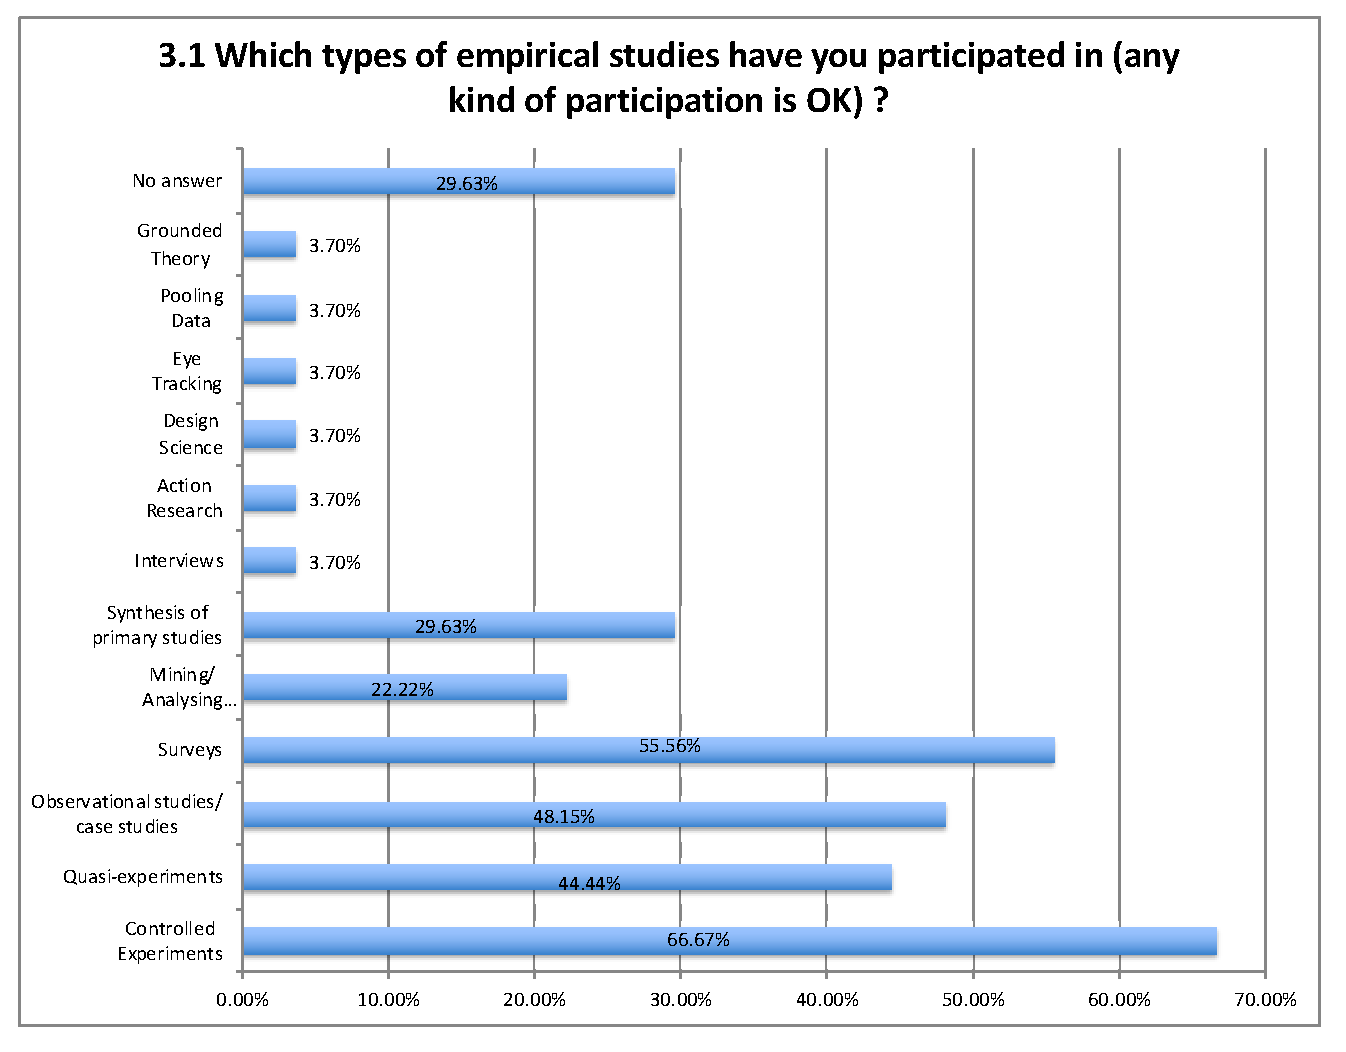
\includegraphics[width=10cm]{Images/Other-Empirical-Methods-SE}
%	\caption{Application of Other Empirical Methods in SE}
%	\label{fig-other-empirical-methods-SE}
%\end{figure*}

\subsection{Experimental training}
La mayor�a de los investigadores encuestados (66.67\%) indican que su formaci�n se bas� en la pr�ctica, y en el aprendizaje de la mano de investigadores con experiencia en el campo. Otras modalidades de formaci�n son cursos formales (59.26\%), auto aprendizaje a partir de textos de experimentaci�n (51.85\%) y de material experimental (48.15\%). El tiempo de formaci�n de los investigadores ha sido variado: el 26\% indican que se han formado al menos por un a�o, el  15\%  entre uno y dos a�os, y la mayor�a (59\%) por m�s de dos a�os. El panorama es bastante similar al observado en el grupo de investigaci�n estudiado; la formaci�n autodidacta es mayoritaria (SR1), y los tiempos de formaci�n son coincidentes, seg�n nos indican los investigadores del GrISE.

Abundando en el tema de la formaci�n de los investigadores, los t�picos abordados son variados. La Figura \ref{fig-topics-training} muestra las tem�ticas espec�ficas reportadas por los investigadores encuestados. Un 45\% de los investigadores coincidi� en haber estudiado el proceso de experimentaci�n, un 22\% indica haber estudiado m�todos emp�ricos tales como: experimentos controlados, replicaci�n de experimentos, estudios de caso, encuestas y revisi�n sistem�tica de literatura. Un menor porcentaje de investigadores (7\%) indican haber recibido formaci�n en dise�o experimental. Es relevante mencionar que un porcentaje considerable de investigadores (19\%) no indican los t�picos en los que se bas� su formaci�n en experimentaci�n. La diversidad de respuestas sugiere que no existe, dentro de SE, una conciencia clara de los conocimientos que un experimentador debe poseer.

\begin{figure*}[htbp!]
	\centering
	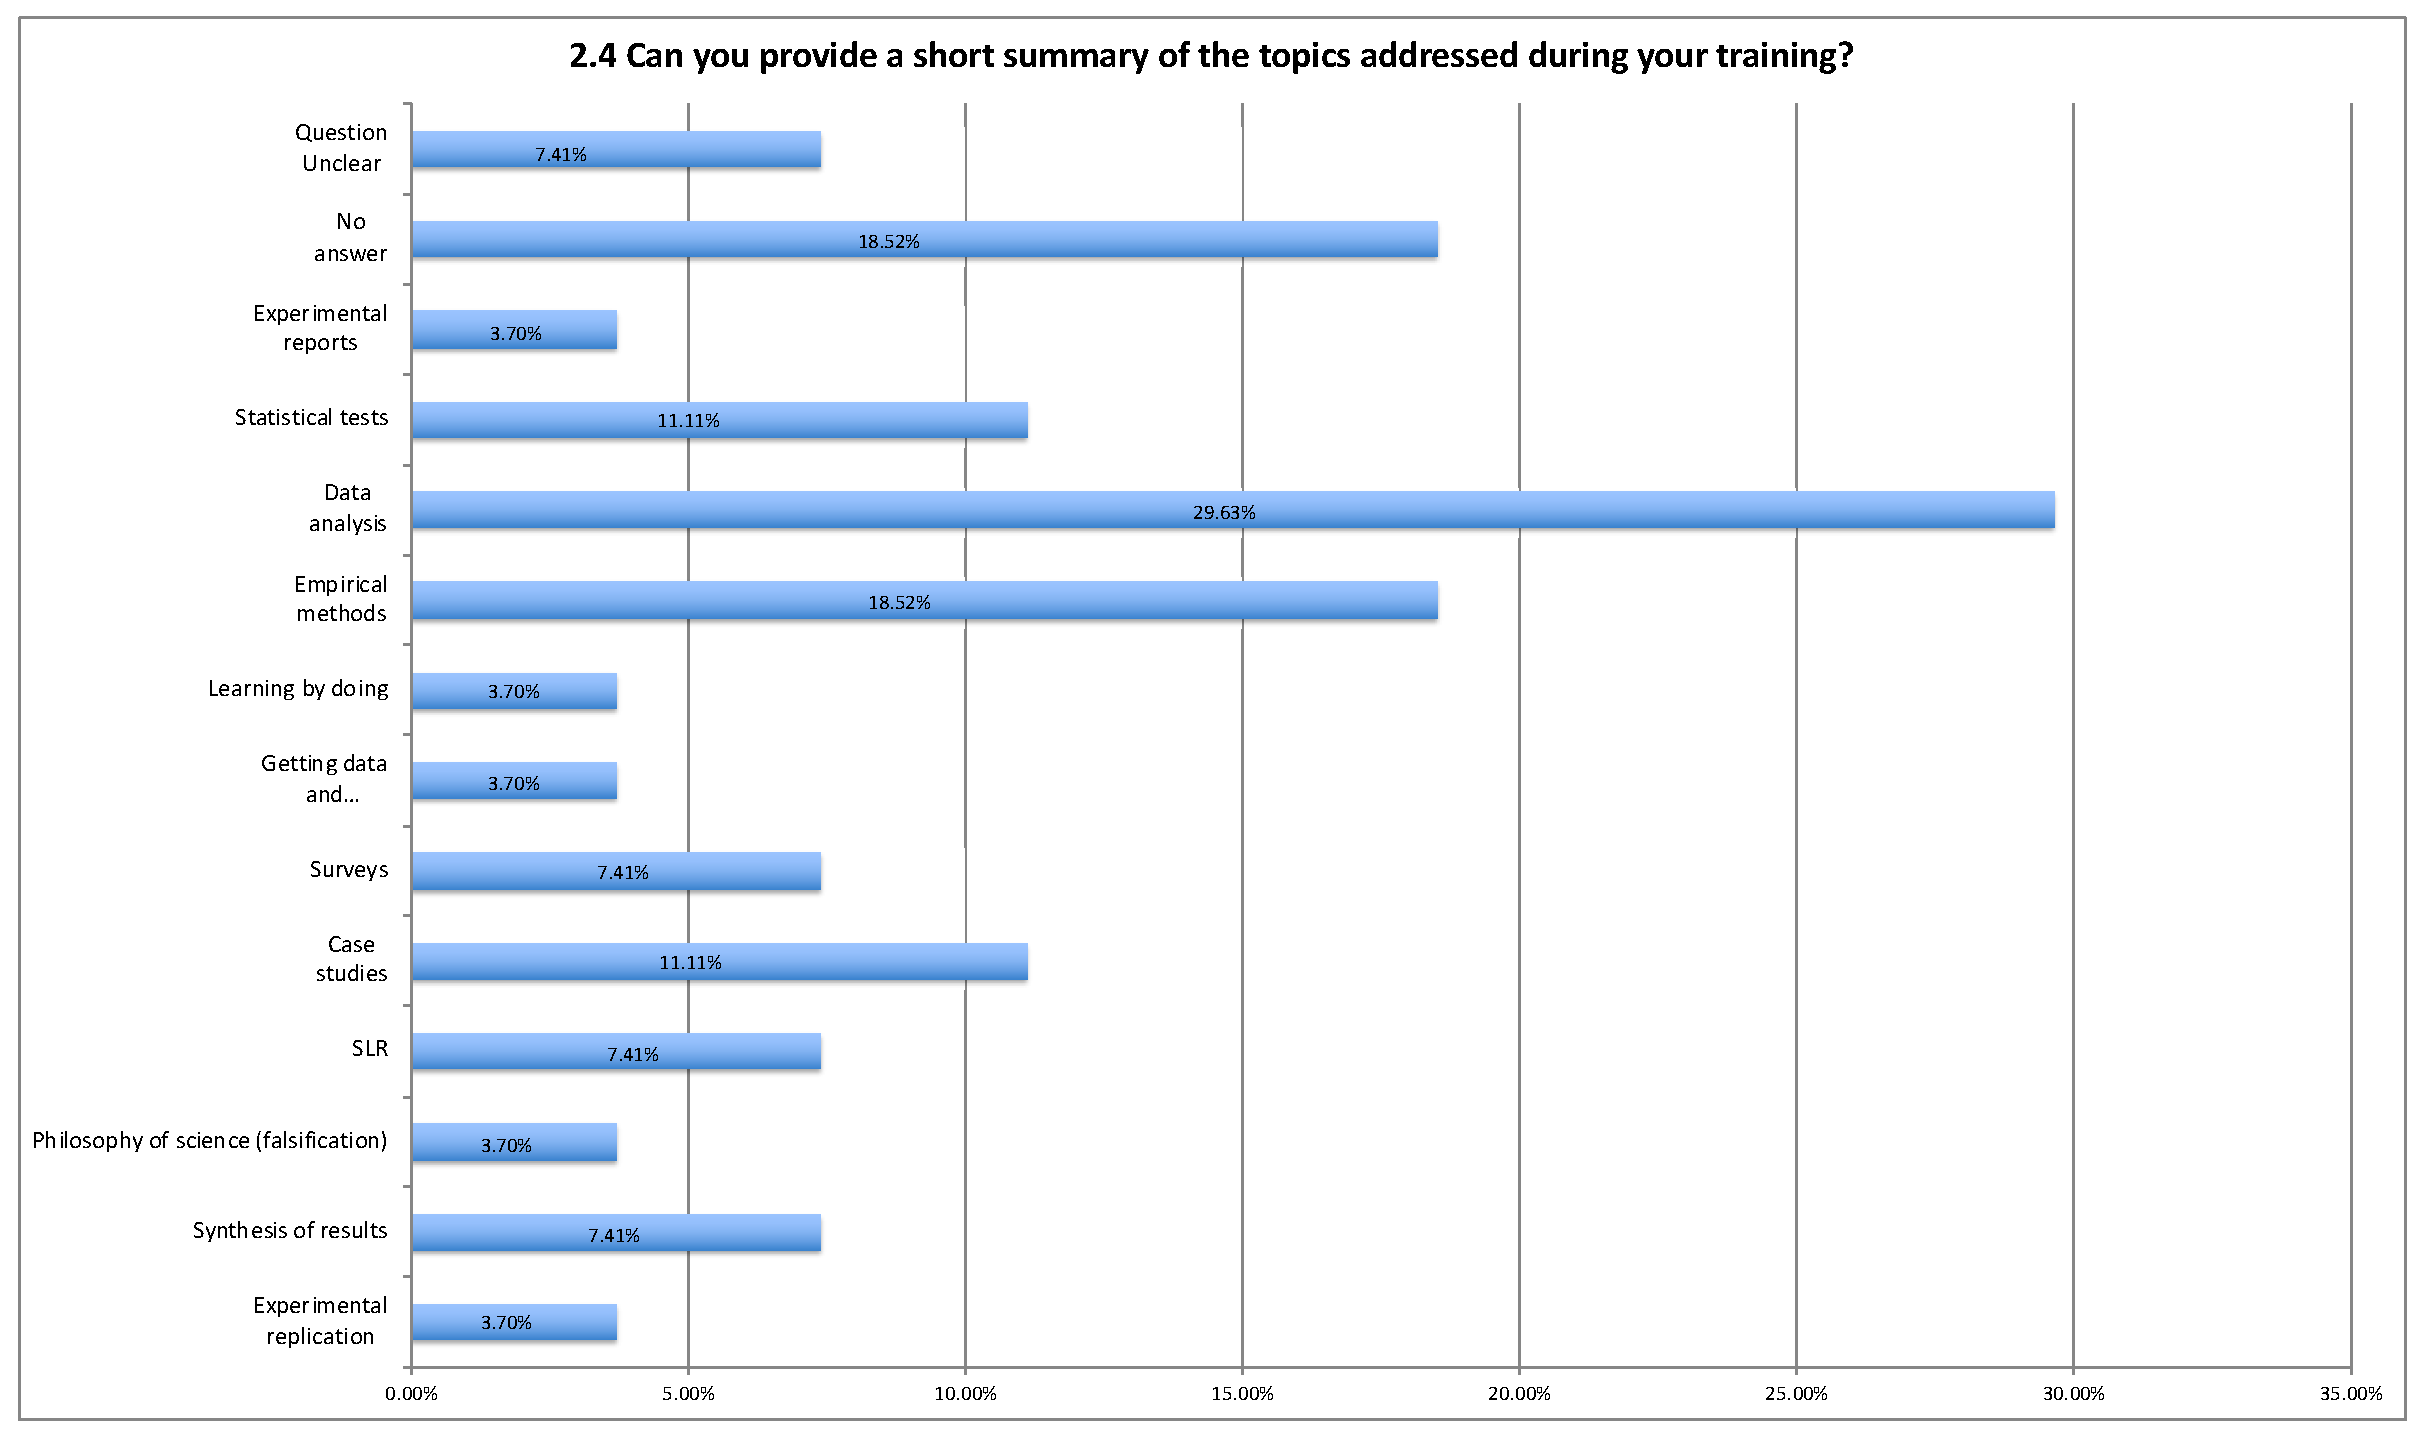
\includegraphics[width=18cm]{Images/Topics-SE-experimentation-training}
	\caption{Topics considered on SE experimentation training}
	\label{fig-topics-training}
\end{figure*}

\subsection{Training materials}
Por training materials, nos referimos a los libros, art�culos, etc., que han sido utilizadas por los investigadores para su formaci�n. La encuesta mostr� que las fuentes usadas son escasas, tal y como muestra la Fig. \ref{fig-resources-training}. Los encuestados indican que el libro de Wohlin et al. \cite{Wohlin2012-Experimentation} es el m�s popular entre los investigadores de SE (67\%), mientras que los libros de Juristo et al. \cite{Juristo-2001-SE-experimentation} y Runenson et al. \cite{Runenson-2012-SE-case-study} le siguen en popularidad en un 15\% de los casos.

\begin{figure*}[htbp!]
	\centering
	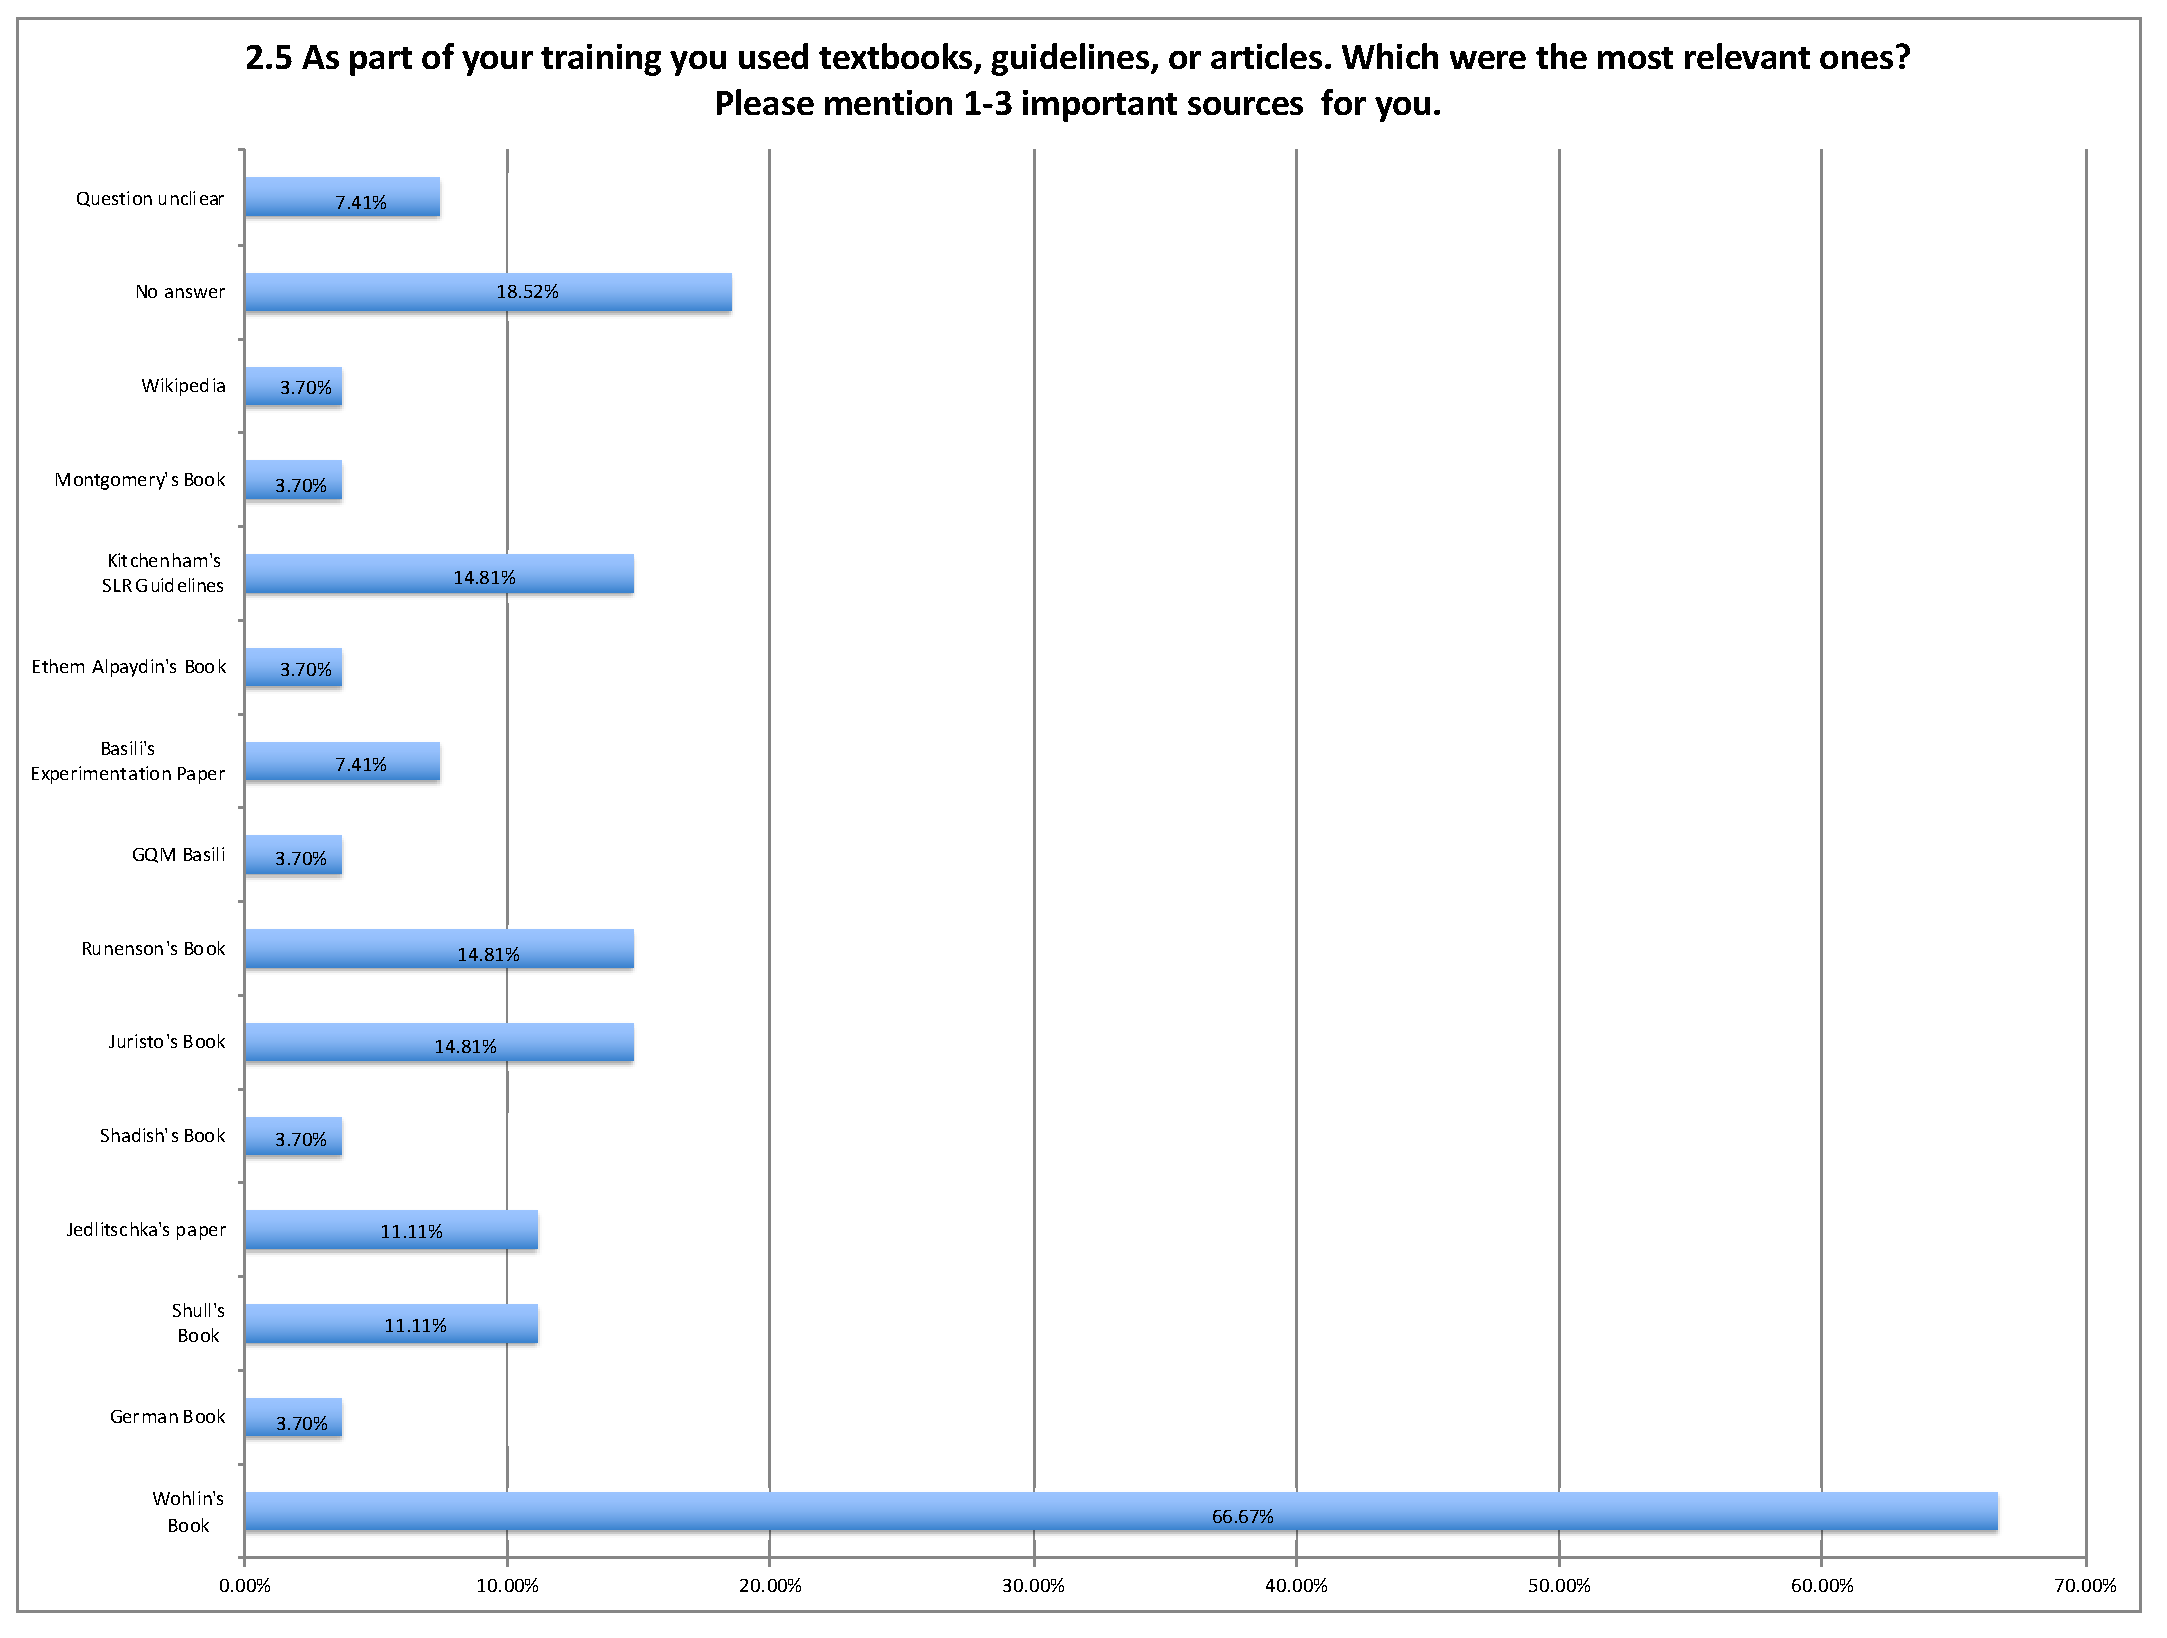
\includegraphics[width=17.5cm]{Images/Experimentation-training-resources}
	\caption{Base materials for learning SE experimentation}
	\label{fig-resources-training}
\end{figure*}

Es preciso indicar que un alto porcentaje de encuestados (29\%) no indica cuales fueron las fuentes utilizadas en su formaci�n en SE experimentation. Esto podr�a justificarse por la utilizaci�n de otras fuentes m�s ligadas a la pr�ctica, como los reportes experimentales o art�culos espec�ficos. A este respecto, hemos preguntado a los investigadores en qu� ha consistido su formaci�n pr�ctica. Casi un 60\% no respondi�, lo cual probablemente indica que la pregunta no estaba bien formulada. A�n as�, el 40\% de respuestas mostradas en la Figura \ref{fig-way-researchers-learn}, muestra que los investigadores aprendieron a experimentar en la pr�ctica principalmente leyendo reportes experimentales notables (25.93\%), tales como the Basili's experimentation paper \cite{Basili-1986-ESE} y the Jedlitschka's experimentation paper \cite{Jedlitschka-2005-GuideLines-ESE}, pidiendo recomendaciones de investigadores expertos en experimentaci�n (18.52\%) y leyendo libros de experimentaci�n de uso cotidiano en la comunidad (14.81\%), tales como The Wohlin's book \cite{Wohlin2012-Experimentation} y The Juristo's book \cite{Juristo-2001-SE-experimentation}. Este resultado est� en concordancia con el resultado SR2 de la etnograf�a de SE, donde se concluy� que las fuentes utilizadas para la formaci�n de los experimentadores en SE son m�ltiples.

\begin{figure*}[htbp!]
	\centering
	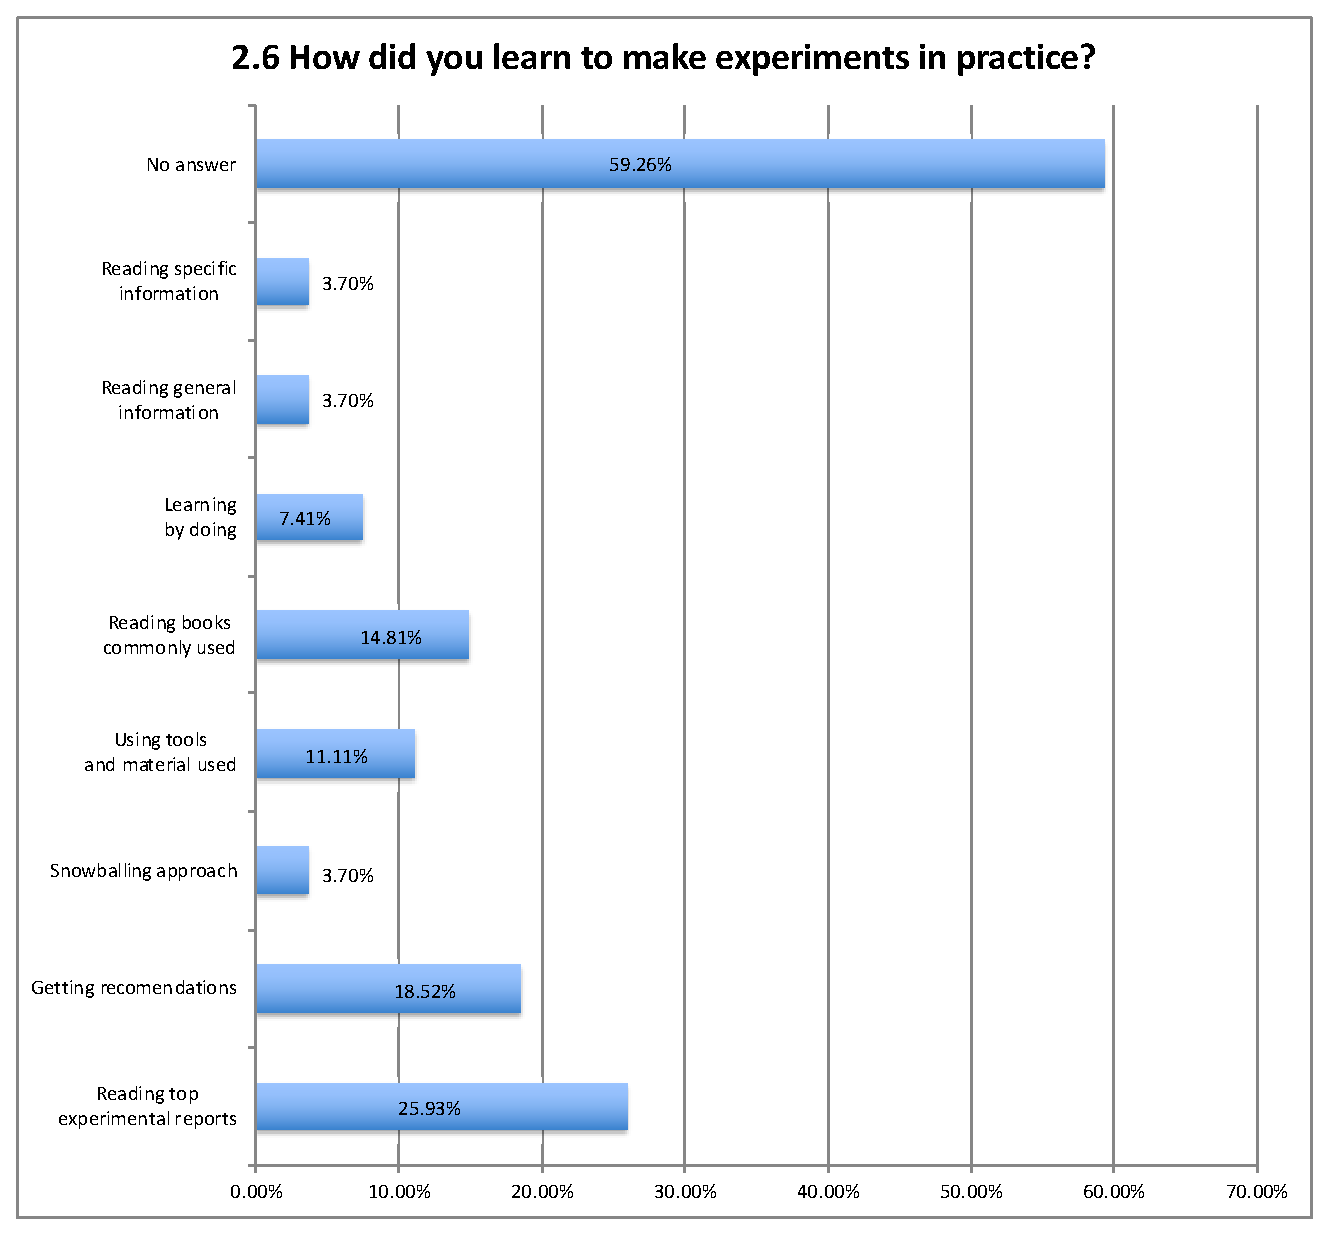
\includegraphics[width=10cm]{Images/Way-researchers-learn-SE-experimentation}
	\caption{The way in which researchers learn SE experimentation}
	\label{fig-way-researchers-learn}
\end{figure*}

\subsection{Terminological diversity}
Los hallazgos obtenidos en el estudio etnogr�fico (SR3) sugieren que la manera en que los investigadores adquirieron el conocimiento de experimentaci�n representa a una de las principales causas de la diversidad conceptual y operativa observada. La variedad en las fuentes y tipos de formaci�n en experimental SE sugieren que la diversidad terminol�gica deber�a aparecer tambi�n en la generalidad de investigadores de experimental SE.

A este respecto, la estrategia que hemos utilizado en el survey ha consistido en indagar sobre ciertos conceptos que consideramos b�sicos, y observar la interpretaci�n que los encuestados hac�an de los mismos. Por ejemplo, cuando se indag� sobre �Qu� palabra usa usted para referirse al proceso donde se definen los detalles del experimento y se eval�an las amenazas a la validez?, el 48\% de encuestados no respondi�, un 26\% cit� el t�rmino \textquotedblleft Planning\textquotedblright, un 18\% a \textquotedblleft Design\textquotedblright, un 4\% a \textquotedblleft Experiment setting\textquotedblright, y un 4\% a \textquotedblleft Guideline\textquotedblright. Solo en muy pocas preguntas de este estilo se not� consenso. Por ejemplo, cuando se pregunt� �Qu� palabra usa para referirse al proceso en el que se estudian los datos experimentales o las m�tricas, probablemente utilizando m�todos estad�sticos?, el 37\% cit� el t�rmino \textquotedblleft Data Analysis\textquotedblright.

Tambi�n fueron planteadas preguntas enfocadas en la conceptualizaci�n de la experimentaci�n. Por ejemplo, cuando se solicit� definir el concepto de: \textquotedblleft Selecci�n de sujetos\textquotedblright, casi un 70\% de los encuestado no respondi�, y del 30\% de respuestas obtenidas, ninguna coincid�a entre s�. Solo en muy pocos conceptos hubo cierto grado de consenso. Por ejemplo, cuando se pidi� a los investigadores encuestados que definieran el concepto: \textquotedblleft Hypothesis formulation\textquotedblright, un 22\% respondi� \textquotedblleft Define testable statistical hypothesis\textquotedblright~y un 11\% \textquotedblleft What to check through the experiment\textquotedblright, lo que representa un alto grado de coincidencia considerando que un 63\% no respondi�. El set de preguntas planteadas puso de manifiesto la existencia de una marcada diversidad conceptual en la comunidad de SE emp�rica.

\subsection{Operational diversity}
Los hallazgos en torno al estudio etnogr�fico muestran que el protocolo seguido en la experimentaci�n dentro de un grupo de investigaci�n en SE no es uniforme. En el survey se plantearon preguntas enfocadas en las actividades que realizan los investigadores de la comunidad de ESE al momento de llevar a cabo un experimento, con el prop�sito de contrastar el estudio etnogr�fico. La Fig. \ref{fig-Operational-Diversity-ESE-Community} muestra las actividades de experimentaci�n con las que se identifican los investigadores de la comunidad ESE. Las respuestas exhiben un alto nivel de coherencia, ya que al final hemos obtenido la descripci�n de procesos experimentales completos. Sin embargo, la diversidad operativa indicada en SR4 se manifiesta claramente debido a que, en lugar de 1 o 2 procesos, hemos obtenido la definici�n de 7 procesos distintos. Las mayores diferencias entre los procesos ocurren a nivel de las actividades de validity evaluation, data set reduction, results documentation y experiment report.

\begin{figure*}[htbp!]
	\centering
	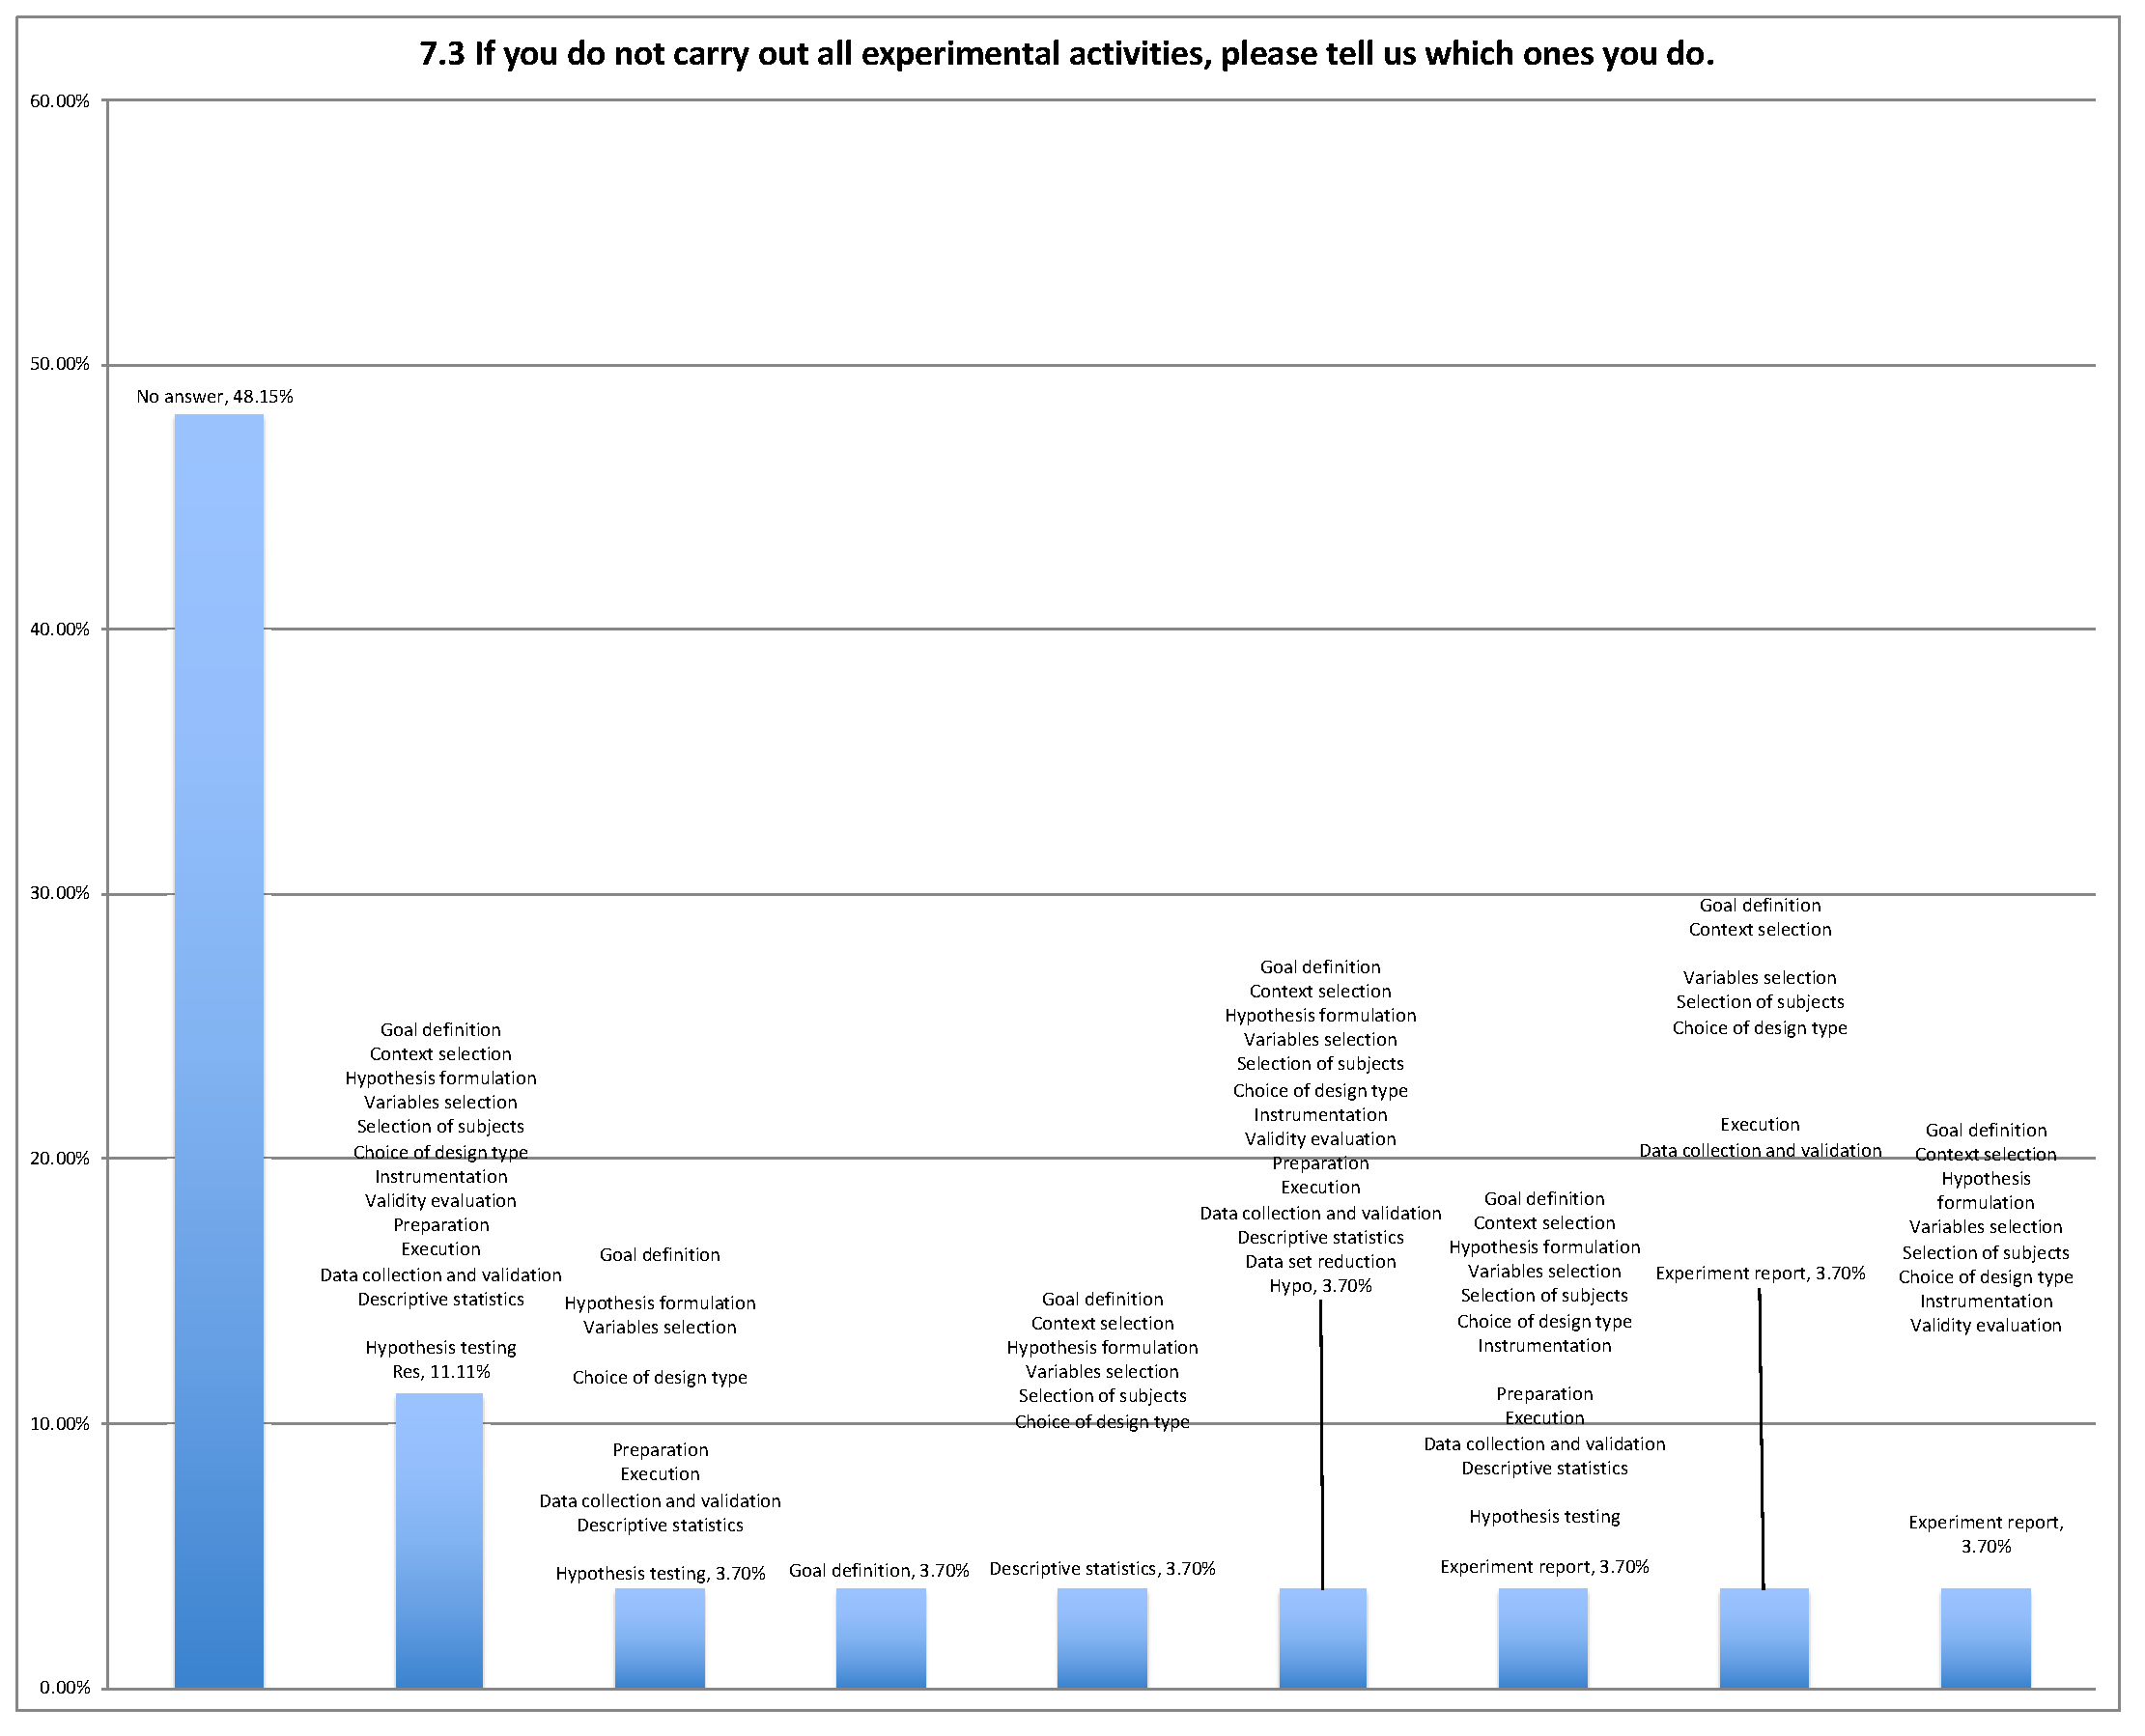
\includegraphics[width=17cm]{Images/Operational-Diversity-ESE-Community}
	\caption{Operational Diversity in Experimentation within the ESE Community}
	\label{fig-Operational-Diversity-ESE-Community}
\end{figure*}

\subsection{Roles}
Un aspecto bastante caracter�stico obtenido en la etnograf�a de SE es la existencia de roles (SR7). Aunque aproximadamente un 48.15\% de los encuestados no respondi� a la pregunta If you do not carry out all experimental activities, please tell us which ones you do?, un 37.04\% indican que no todas las actividades de experimentaci�n son llevadas a cabo por un solo investigador, lo cual es corroborado por un 33.33\% que indican que la complejidad del proceso de experimentaci�n define roles, e incluso un 29.63\% concuerda en que las actividades realizadas son distribuidas de acuerdo con las habilidades o conocimiento de los investigadores.



%Finalmente, encontramos que al parecer para los investigadores encuestados no es del todo claro el prop�sito de la SE experimentation. Aunque la mayor�a de investigadores encuestados (62.96\%) indican que la experimentaci�n esta orientada a la creaci�n de conocimiento en base a datos emp�ricos y a m�ltiples replicaciones para ser transferido a la industria y a la academia; no obstante, un 33.33\% no indican cual es el prop�sito de hacer experimentos en SE, de la mano de otro 25.93\% que tambi�n responde que los experimentos sirven para ganar conocimiento acerca de un fen�meno bajo estudio y para publicar eventualmente los resultados de experimentos aislados (ver Fig. \ref{Purpose-SE-Experiments}).

%\begin{figure*}[htbp!]
%	\centering
%	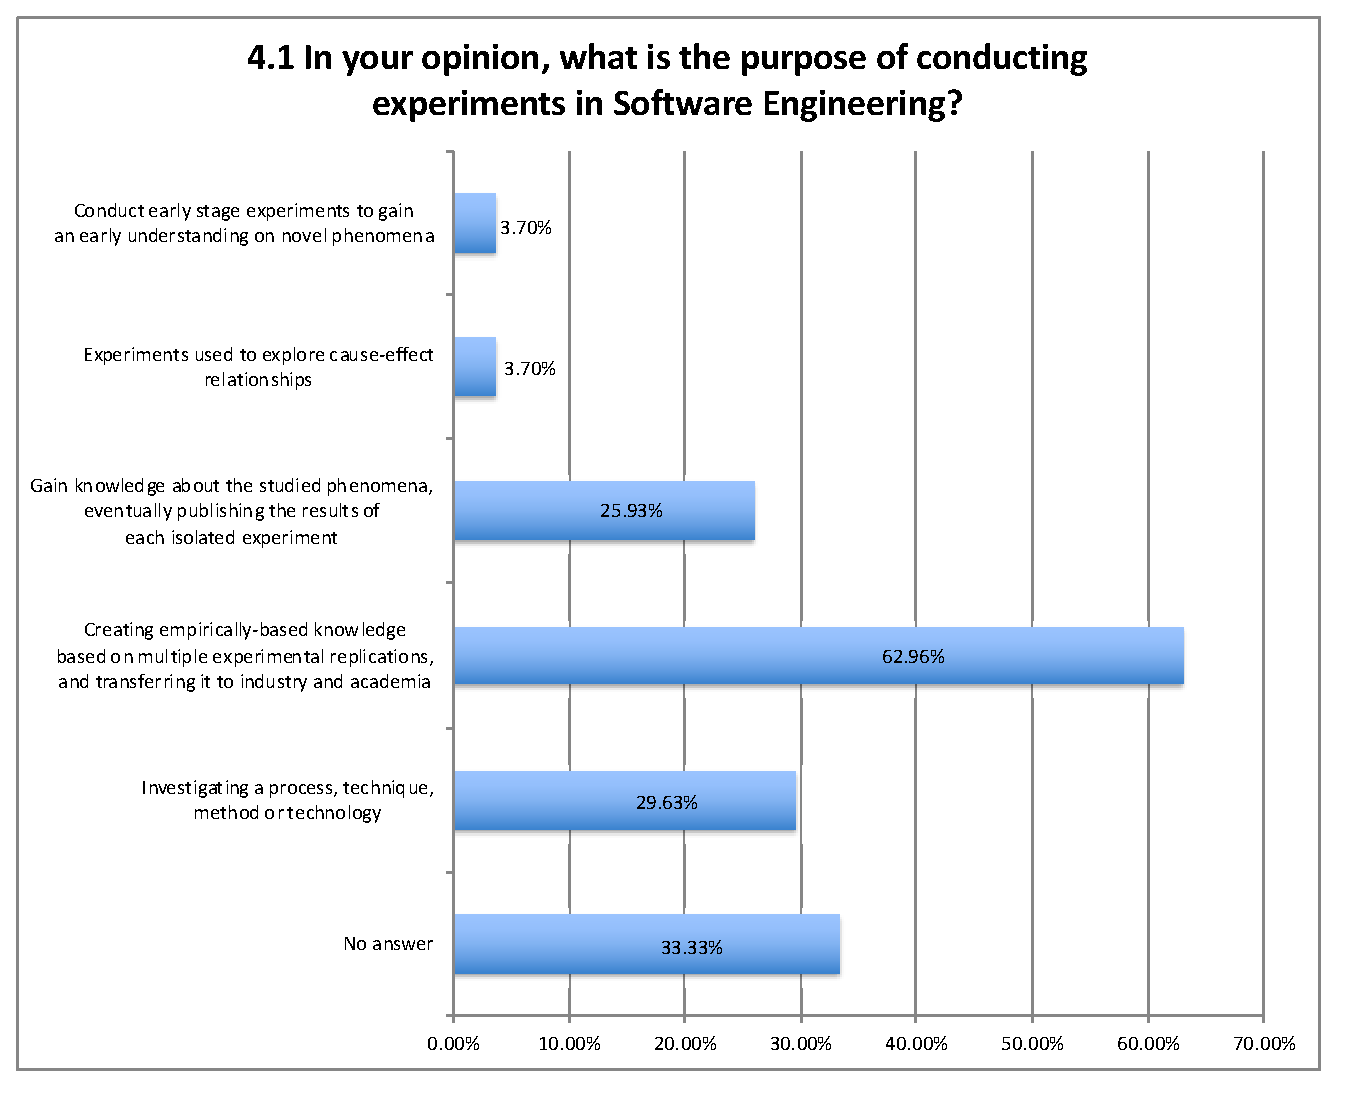
\includegraphics[width=12cm]{Images/Purpose-SE-Experiments}
%	\caption{Purpose of SE Experiments}
%	\label{fig-Purpose-SE-Experiments}
%\end{figure*}

%Esta situaci�n se corrobor� al indagar sobre las situaciones en las cuales un experimento es seleccionado como m�todo de investigaci�n (ver Fig. \ref{fig-why-experiments-done}), lo que no fue respondido por un 40.74\% de los encuestados. No obstante, quienes respondieron tuvieron criterios divididos: Un 18.52\% dijo que un experimento se realiza para aislar un fen�meno de inter�s o para confirmar un tipo espec�fico de hip�tesis; mientras que un 14.81\% indic� que se utiliza para comparar dos cosas o para investigar una relaci�n causa-efecto. Minoritariamente hubo investigadores que indicaron que un experimento se realiza dependiendo de la pregunta de investigaci�n planteada (11.11\%), como prueba de concepto (3.7\%) y cuando una replicaci�n es posible (3.7\%).

%\begin{figure*}[htbp!]
%	\centering
%	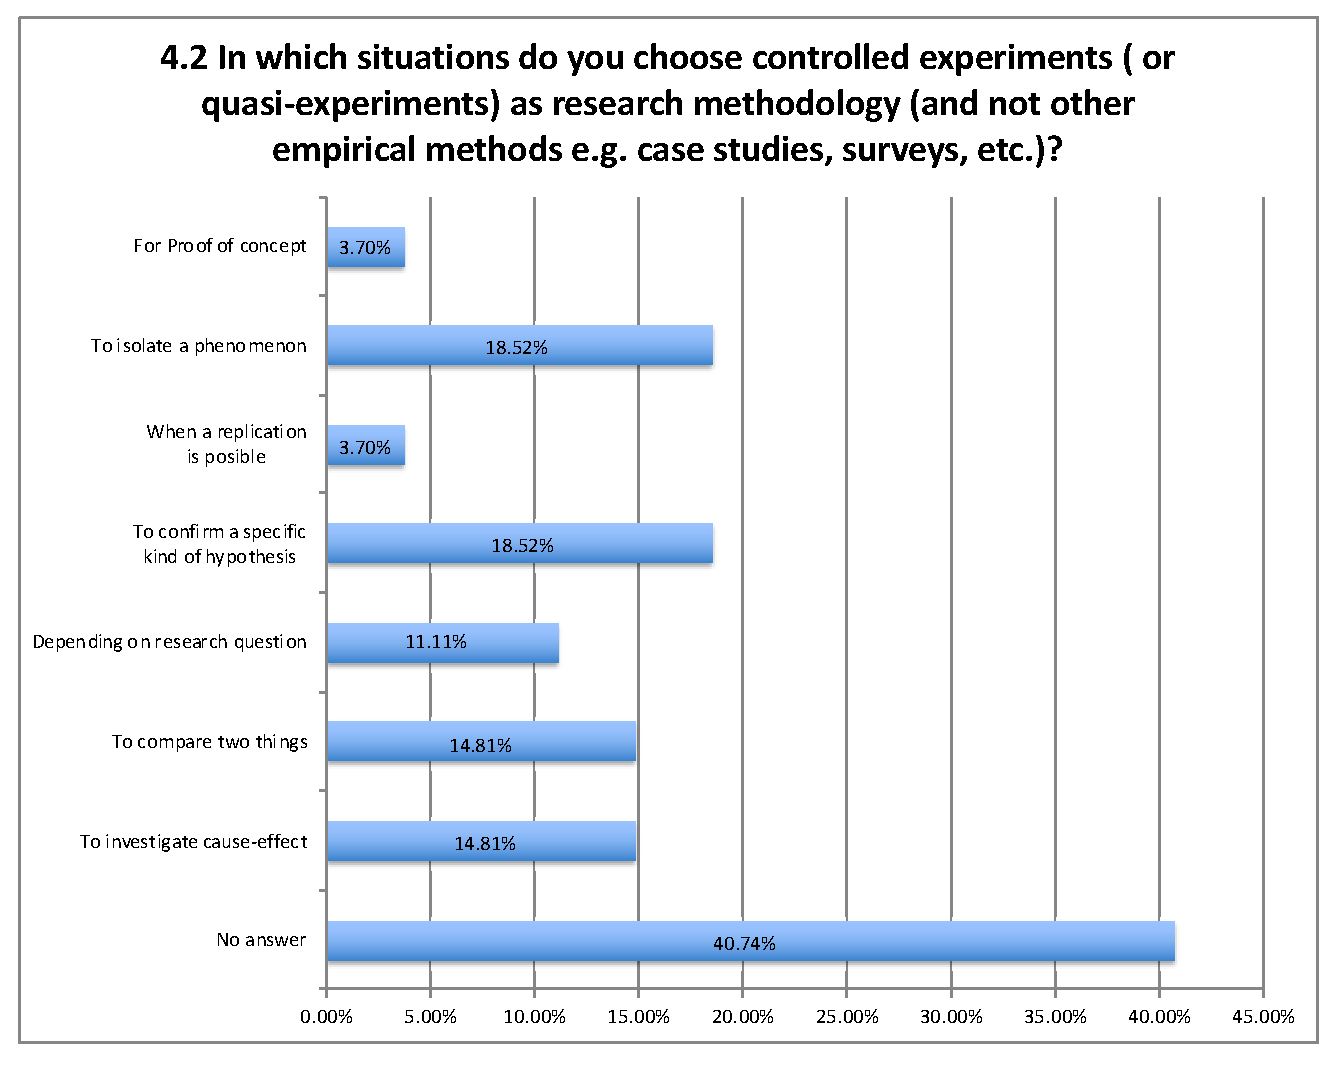
\includegraphics[width=12cm]{Images/Why-Experiment-Method-Selected}
%	\caption{Reasons why an Experiment is Selected as Research Method}
%	\label{fig-why-experiments-done}
% \end{figure*}

\subsection{Conclusiones}
Los resultados del survey han demostrado en gran medida que los hallazgos del estudio etnogr�fico que hemos realizado dentro de un grupo de investigaci�n en ESE son generalizables a la comunidad de ESE:

\begin{enumerate}[label={SrR\arabic*)}]
\item \textbf{Educaci�n:} La formaci�n en experimentaci�n de los investigadores en ESE ha sido informal: tiempos de entrenamiento variados, aprendizaje obtenido a partir de distintas fuentes y con contenidos muy variados. En la mayor�a de los casos, la formaci�n ha tenido una componente eminentemente pr�ctica.

\item \textbf{Fuentes:} Las fuentes de informaci�n utilizadas en la comunidad de ESE son generales y escasas.  El texto m�s popular en la comunidad es el libro de Wohlin et al \cite{Wohlin2000}, seguido de Juristo et al. \cite{Juristo-2001-SE-experimentation} y Runenson et al. \cite{Runenson-2012-SE-case-study}.

\item \textbf{Terminologia:} Los investigadores en ESE utilizan una terminolog�a muy variada para referirse a las fases del proceso experimental. 

\item \textbf{Operaci�n:} No existe un �nico proceso experimental, sino varios procesos compuestos de distintas etapas.
	
\item \textbf{Roles:} Los investigadores en ESE no son polivalentes. Asumen roles en el proceso experimental dependiendo de sus conocimientos y experiencia.
\end{enumerate}

\section{Discussion and Conclusions}\label{sec-discussion-conclusions}
\subsection{Issues surrounding SE experimentation}
El estudio etnogr�fico devel� varias situaciones problem�ticas en torno a la experimentaci�n en SE, particularmente en lo referente a la comunicaci�n debida a la diversidad terminol�gica y operativa existente en el grupo de investigaci�n estudiado. El survey abord� m�s expl�citamente la problem�tica en torno a la experimentaci�n en la comunicad de ESE. Encontramos que m�s de un 60\% de los investigadores encuestados consideran que la experimentaci�n en SE es compleja debido a distintos factores (ver Fig. \ref{fig-Factors-Influencing-Complexity-ESE}). Por ejemplo, un 33.33\% considera que la complejidad de la experimentaci�n se debe a que el {\color{green}(SC9)} \ul{low sample size results in weak arguments which avoid addressing the industrial problems}; mientras que un 11\% cree que {\color{green}(SC10)} \ul{the abundant range of statistical tests options and poor knowledge about it results in an erroneous statistical study}.

\begin{figure*}[htbp!]
	\centering
	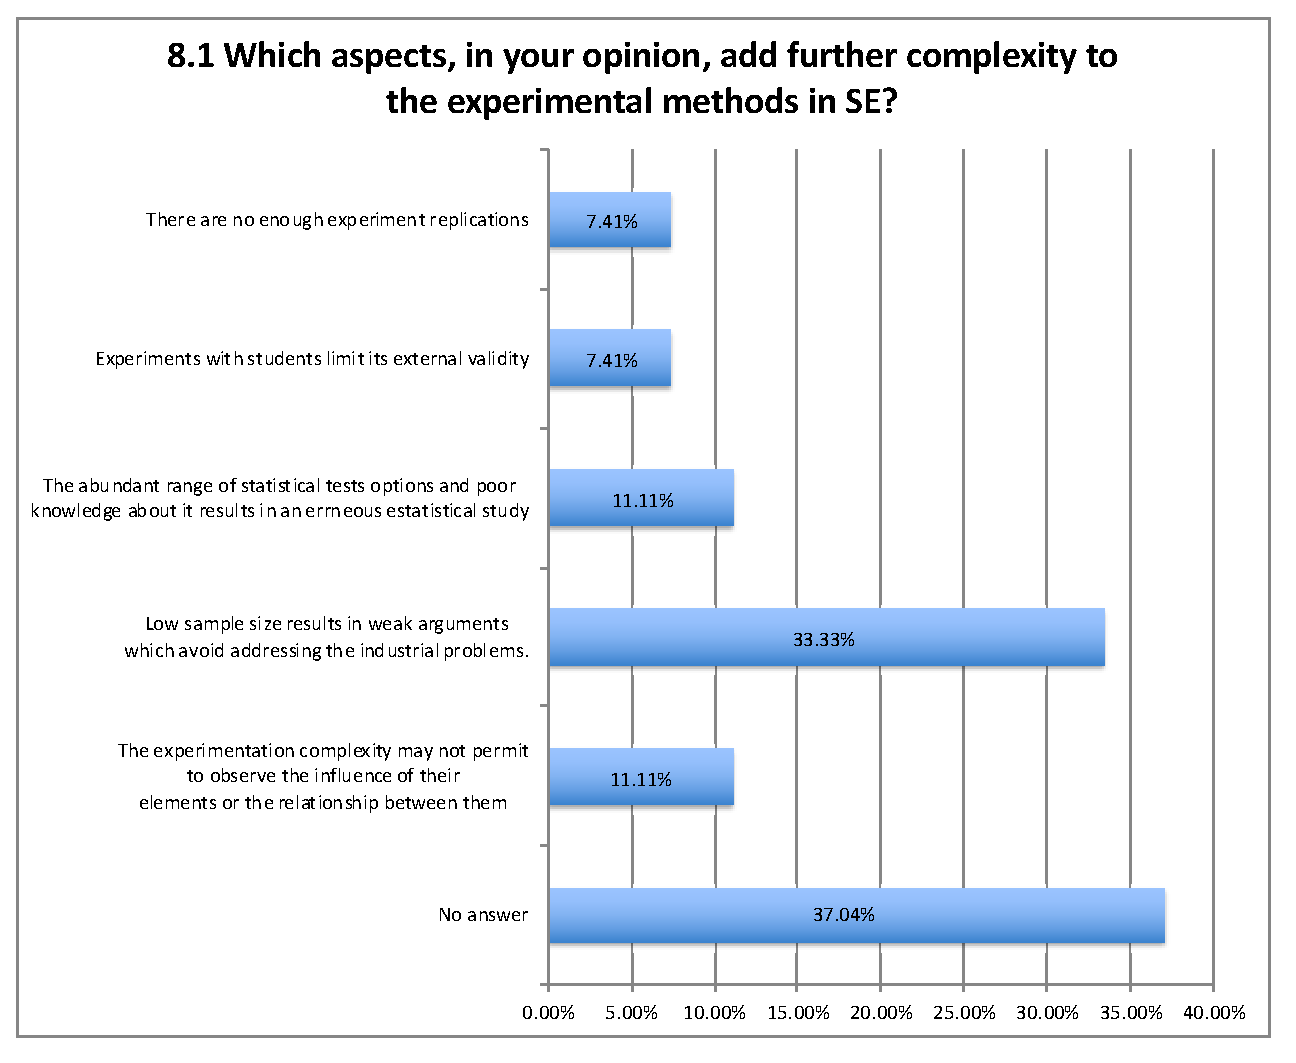
\includegraphics[width=12cm]{Images/Factors-Influencing-Complexity-ESE}
	\caption{Factors influencing the complexity of experimentation in SE}
	\label{fig-Factors-Influencing-Complexity-ESE}
\end{figure*}

As� mismo, un 11\% de los investigadores piensan que {\color{green}(SC11)} \ul{the experimentation complexity may not permit to observe the influence of their elements or the relationship between them}; mientras que otros investigadores son m�s espec�ficos y le atribuyen la complejidad de la experimentaci�n a que {\color{green}(SC12)} \ul{there are no enough experiment replications} (7.41\%) y a que los {\color{green}(SC13)} \ul{experiments with students limit its external validity} (7.41\%).

Por otra parte, otro problema remarcado en este estudio es el referido a la dificultad en la gesti�n de los datos. Un 14.81\% considera que {\color{green}(SC14)} \ul{el manejo y el an�lisis de los datos experimentales son complejos, lo que podr�a deberse en parte a las distintas maneras que tienen los investigadores para gestionarlos}: Un 66.67\% afirma que utilizan hojas de calculo, un 25\% repositorios de datos relacionales y un 44\% formatos propietarios. Por otra parte, un 7.41\% de los encuestados hace �nfasis en la limitada compartici�n de datos que existe, lo que es corroborado por mas de un 10\% de investigadores que consideran que {\color{green}(SC15)} \ul{la agregaci�n de datos entre replicaciones es compleja, quiz� en parte porque no existe un soporte adecuado para las replicaciones y la existencia del conocimiento t�cito}.

\begin{tcolorbox}

los aspectos que consideramos como problem�ticos en torno a la SE experimentation fueron corroborados en gran medida por los encuestados, e incluso se obtuvieron importantes recomendaciones a ser consideradas (ver Fig. \ref{fig-recommendations-improve-SE-experimentation}):

\begin{itemize}
  \item To have a common empirical source of knowledge
  \item To use simple guidelines to report findings
  \item To formalize the process
  \item To formalize the terminology
  \item To apply statistical test depending on experiment design
  \item To have a set of selected experimental subjects
  \item To receive quality formal courses
\end{itemize}

\end{tcolorbox}

\begin{figure*}[htbp!]
	\centering
	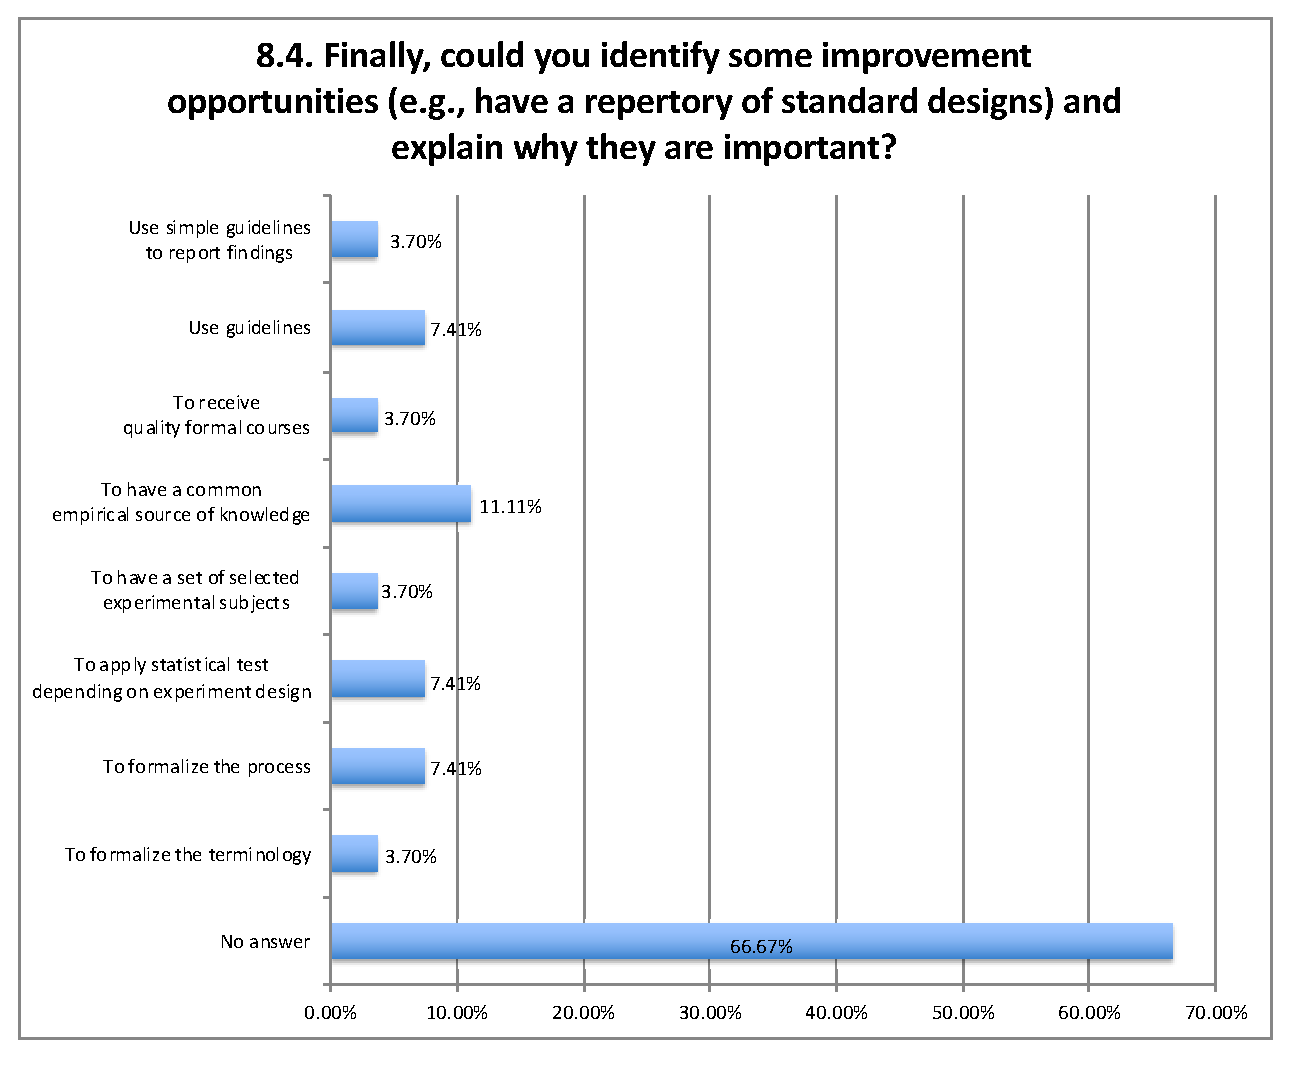
\includegraphics[width=12cm]{Images/Recommendations-Improve-SE-Experimentation}
	\caption{Recommendations to Improve the Experimentation in SE}
	\label{fig-recommendations-improve-SE-experimentation}
\end{figure*}



% Please add the following required packages to your document preamble:
% \usepackage{graphicx}
% \usepackage{lscape}
\begin{landscape}
\begin{table}[]
\centering
\resizebox{\textwidth}{!}{%
\begin{tabular}{rlll}
\hline
\# & Hallazgos del estudio en SE & Hallazgos del estudio en biotecnologia & \# \\ \hline
39 & Existe literatura est�ndar, e.g., \textbackslash{}cite\{Wohlin2000,Juristo2001\} &  &  \\
40 & La carencia de literatura est�ndar se suple con reportes o art�culos espec�ficos, e.g., \textbackslash{}cite\{Basili-1986-ESE\} &  &  \\
 2 & Se produce diversidad terminol�gica entre fuentes &  &  \\
 5 & Existen pocos libros de referencia acerca de experimentaci�n en SE &  &  \\
12 & No existe una pol�tica para la gesti�n del material, o herramientas especializadas &  &  \\
 &  &  & 
\end{tabular}%
}
\caption{Comparaci�n de los hallazgos en SE y Biotecnologia}
\label{tab:comparison}
\end{table}
\end{landscape}





%%%%%%%%%%%%%%%%
%%%%%%%%%%%%%%%%
%\begin{table}
%\centering
%\caption{Frequency of Special Characters}
%\begin{tabular}{|c|c|l|} \hline
%Non-English or Math&Frequency&Comments\\ \hline
%\O & 1 in 1,000& For Swedish names\\ \hline
%$\pi$ & 1 in 5& Common in math\\ \hline
%\$ & 4 in 5 & Used in business\\ \hline
%$\Psi^2_1$ & 1 in 40,000& Unexplained usage\\
%\hline\end{tabular}
%\end{table}
%%%%%%%%%%%%%%%%
%%%%%%%%%%%%%%%%



%%%%%%%%%%%%%%%%
%%%%%%%%%%%%%%%%
%\begin{table*}
%\centering
%\caption{Some Typical Commands}
%\begin{tabular}{|c|c|l|} \hline
%Command&A Number&Comments\\ \hline
%\texttt{{\char'134}alignauthor} & 100& Author alignment\\ \hline
%\texttt{{\char'134}numberofauthors}& 200& Author enumeration\\ \hline
%\texttt{{\char'134}table}& 300 & For tables\\ \hline
%\texttt{{\char'134}table*}& 400& For wider tables\\ \hline\end{tabular}
%\end{table*}
% end the environment with {table*}, NOTE not {table}!
%%%%%%%%%%%%%%%%
%%%%%%%%%%%%%%%%



%%%%%%%%%%%%%%%%
%%%%%%%%%%%%%%%%
%\begin{figure}
%\centering
%\includegraphics[height=1in, width=1in]{images/fly}
%\caption{A sample black and white graphic
%that has been resized with the \texttt{includegraphics} command.}
%\end{figure}
%%%%%%%%%%%%%%%%
%%%%%%%%%%%%%%%%


%%%%%%%%%%%%%%%%
%%%%%%%%%%%%%%%%
%\begin{figure*}
%\centering
%\includegraphics{images/flies}
%\caption{A sample black and white graphic
%that needs to span two columns of text.}
%\end{figure*}
%%%%%%%%%%%%%%%%
%%%%%%%%%%%%%%%%

%%%%%%%%%%%%%%%%
%%%%%%%%%%%%%%%%
%\begin{figure}
%\centering
%\includegraphics[height=1in, width=1in]{images/rosette}
%\caption{A sample black and white graphic that has
%been resized with the \texttt{includegraphics} command.}
%\vskip -6pt
%\end{figure}
%%%%%%%%%%%%%%%%
%%%%%%%%%%%%%%%%
%\
%ACKNOWLEDGMENTS are optional
\section{Acknowledgments}
This section is optional; it is a location for you
to acknowledge grants, funding, editing assistance and
what have you.  In the present case, for example, the
authors would like to thank Gerald Murray of ACM for
his help in codifying this \textit{Author's Guide}
and the \textbf{.cls} and \textbf{.tex} files that it describes.

%
% The following two commands are all you need in the
% initial runs of your .tex file to
% produce the bibliography for the citations in your paper.
\bibliographystyle{abbrv}
\bibliography{Bibliografia}  % sigproc.bib is the name of the Bibliography in this case
% You must have a proper ".bib" file
%  and remember to run:
% latex bibtex latex latex
% to resolve all references
%
% ACM needs 'a single self-contained file'!
%
%APPENDICES are optional
%\balancecolumns
%\appendix
%Appendix A
%\section{Headings in Appendices}
%The rules about hierarchical headings discussed above for
%the body of the article are different in the appendices.
%In the \textbf{appendix} environment, the command
%\textbf{section} is used to
%indicate the start of each Appendix, with alphabetic order
%designation (i.e. the first is A, the second B, etc.) and
%a title (if you include one).  So, if you need
%hierarchical structure
%\textit{within} an Appendix, start with \textbf{subsection} as the
%highest level. Here is an outline of the body of this
%document in Appendix-appropriate form:
%\subsection{Introduction}
%\subsection{The Body of the Paper}
%\subsubsection{Type Changes and  Special Characters}
%\subsubsection{Math Equations}
%\paragraph{Inline (In-text) Equations}
%\paragraph{Display Equations}
%\subsubsection{Citations}
%\subsubsection{Tables}
%\subsubsection{Figures}
%\subsubsection{Theorem-like Constructs}
%\subsubsection*{A Caveat for the \TeX\ Expert}
%\subsection{Conclusions}
%\subsection{Acknowledgments}
%\subsection{Additional Authors}
%This section is inserted by \LaTeX; you do not insert it.
%You just add the names and information in the
%\texttt{{\char'134}additionalauthors} command at the start
%of the document.
%\subsection{References}
%Generated by bibtex from your ~.bib file.  Run latex,
%then bibtex, then latex twice (to resolve references)
%to create the ~.bbl file.  Insert that ~.bbl file into
%the .tex source file and comment out
%the command \texttt{{\char'134}thebibliography}.
% This next section command marks the start of
% Appendix B, and does not continue the present hierarchy
%\section{More Help for the Hardy}
%The sig-alternate.cls file itself is chock-full of succinct
%and helpful comments.  If you consider yourself a moderately
%experienced to expert user of \LaTeX, you may find reading
%it useful but please remember not to change it.
%\balancecolumns % GM June 2007
% That's all folks!
\end{document}
